\chapter{Manufacturing}

If you try to think of any man-made object, whether it was made from woods, metals, or plastics, chances are it was produced through a manufacturing process.

Over time, these processes have been refined to be more efficient, cost-effective, and faster at producing the goods that we use on a daily basis.

New methods are also constantly being developed by engineers and scientists, and today the range of options available means that choosing the most appropriate manufacturing method involves finding the sweet spot between cost-effectiveness, yield, and time needed.

\section{Woods and Metals Processes}

Manufacturing methods that are able to process woods and metals are typically the processes that are used to construct the vast majority of the built world around us. 

Infrastructure, transportation methods, and buildings would not exist without the advent of processes that allow us to accurately machine raw woods and metals into our desired forms.

The following sections will cover methods used to process both material types.

\section{Milling}

Mills are powerful tools that allows us to carve out complex shapes from blocks of raw material. A tool bit follows a path to remove the desired material, which makes it a \newterm{subtractive} manufacturing process. The tool bit itself rotates at a very high speed, which allows for it to process harder materials such as woods and metals.

% graphic outlining how a mill removes material - show a block of raw material, the tool bit with a rotation arrow indicating that it rotates, the tool path, and the milled result
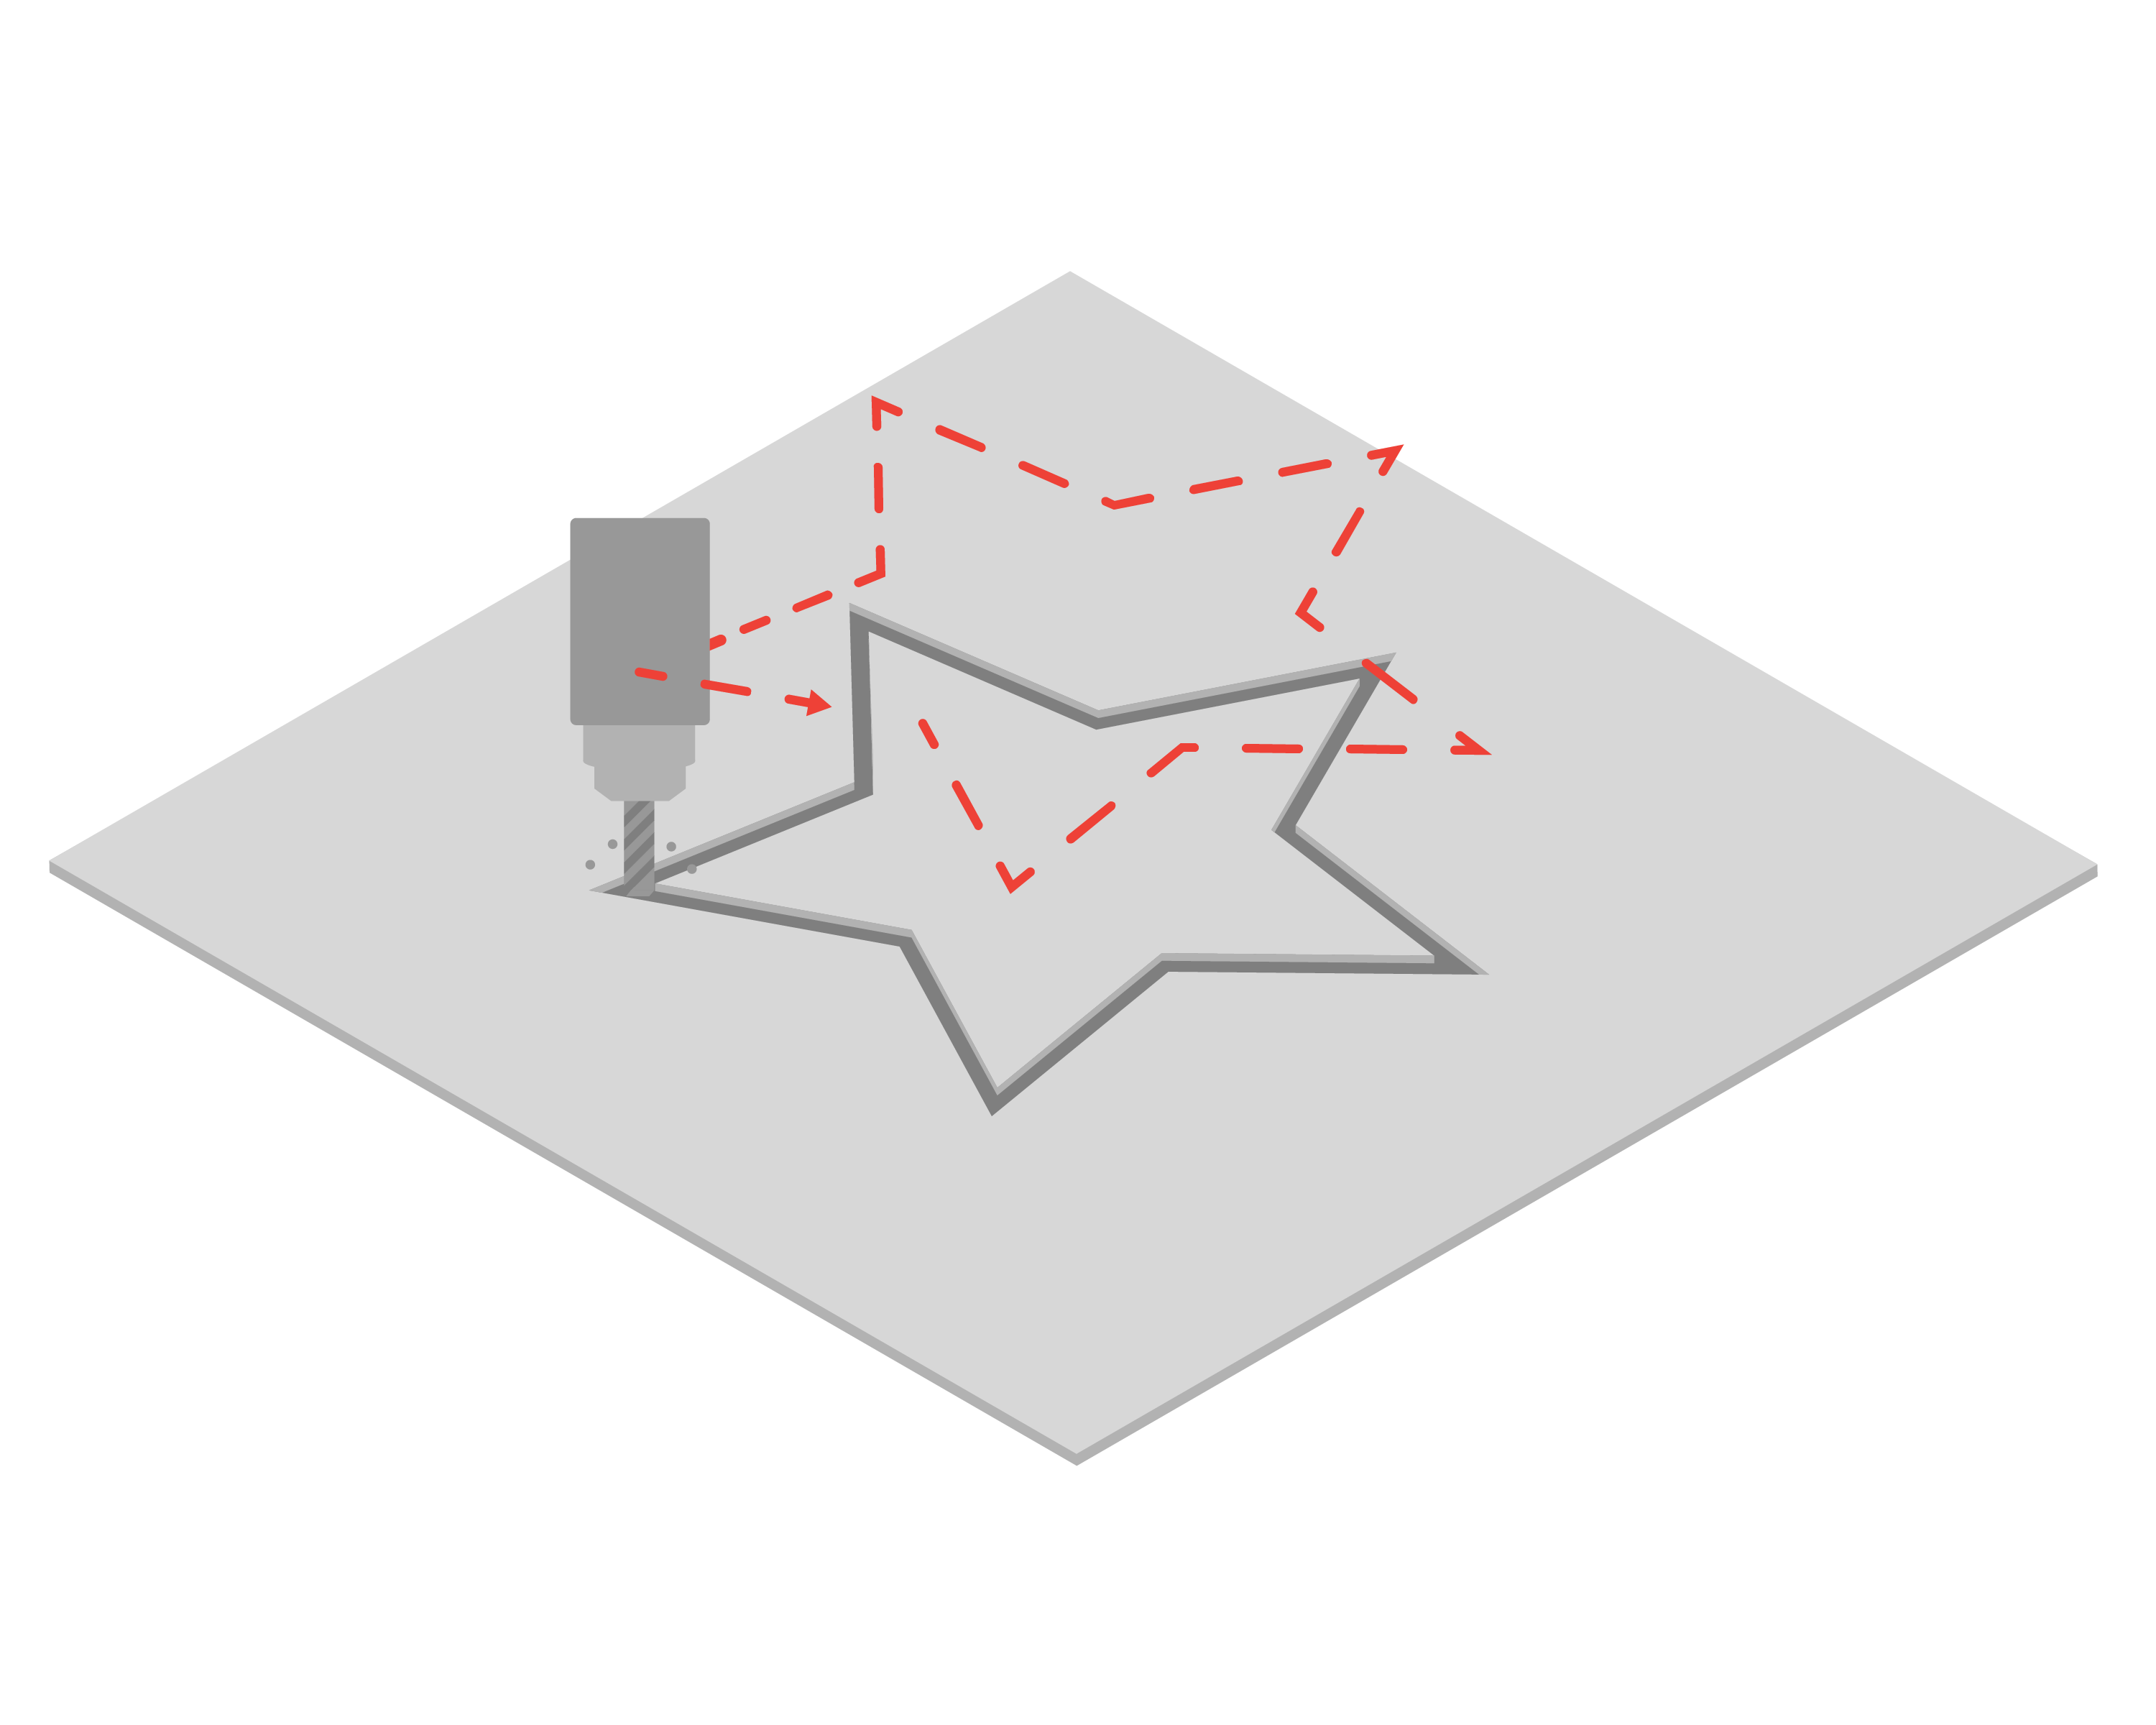
\includegraphics[width=.75\textwidth]{millWide.png}

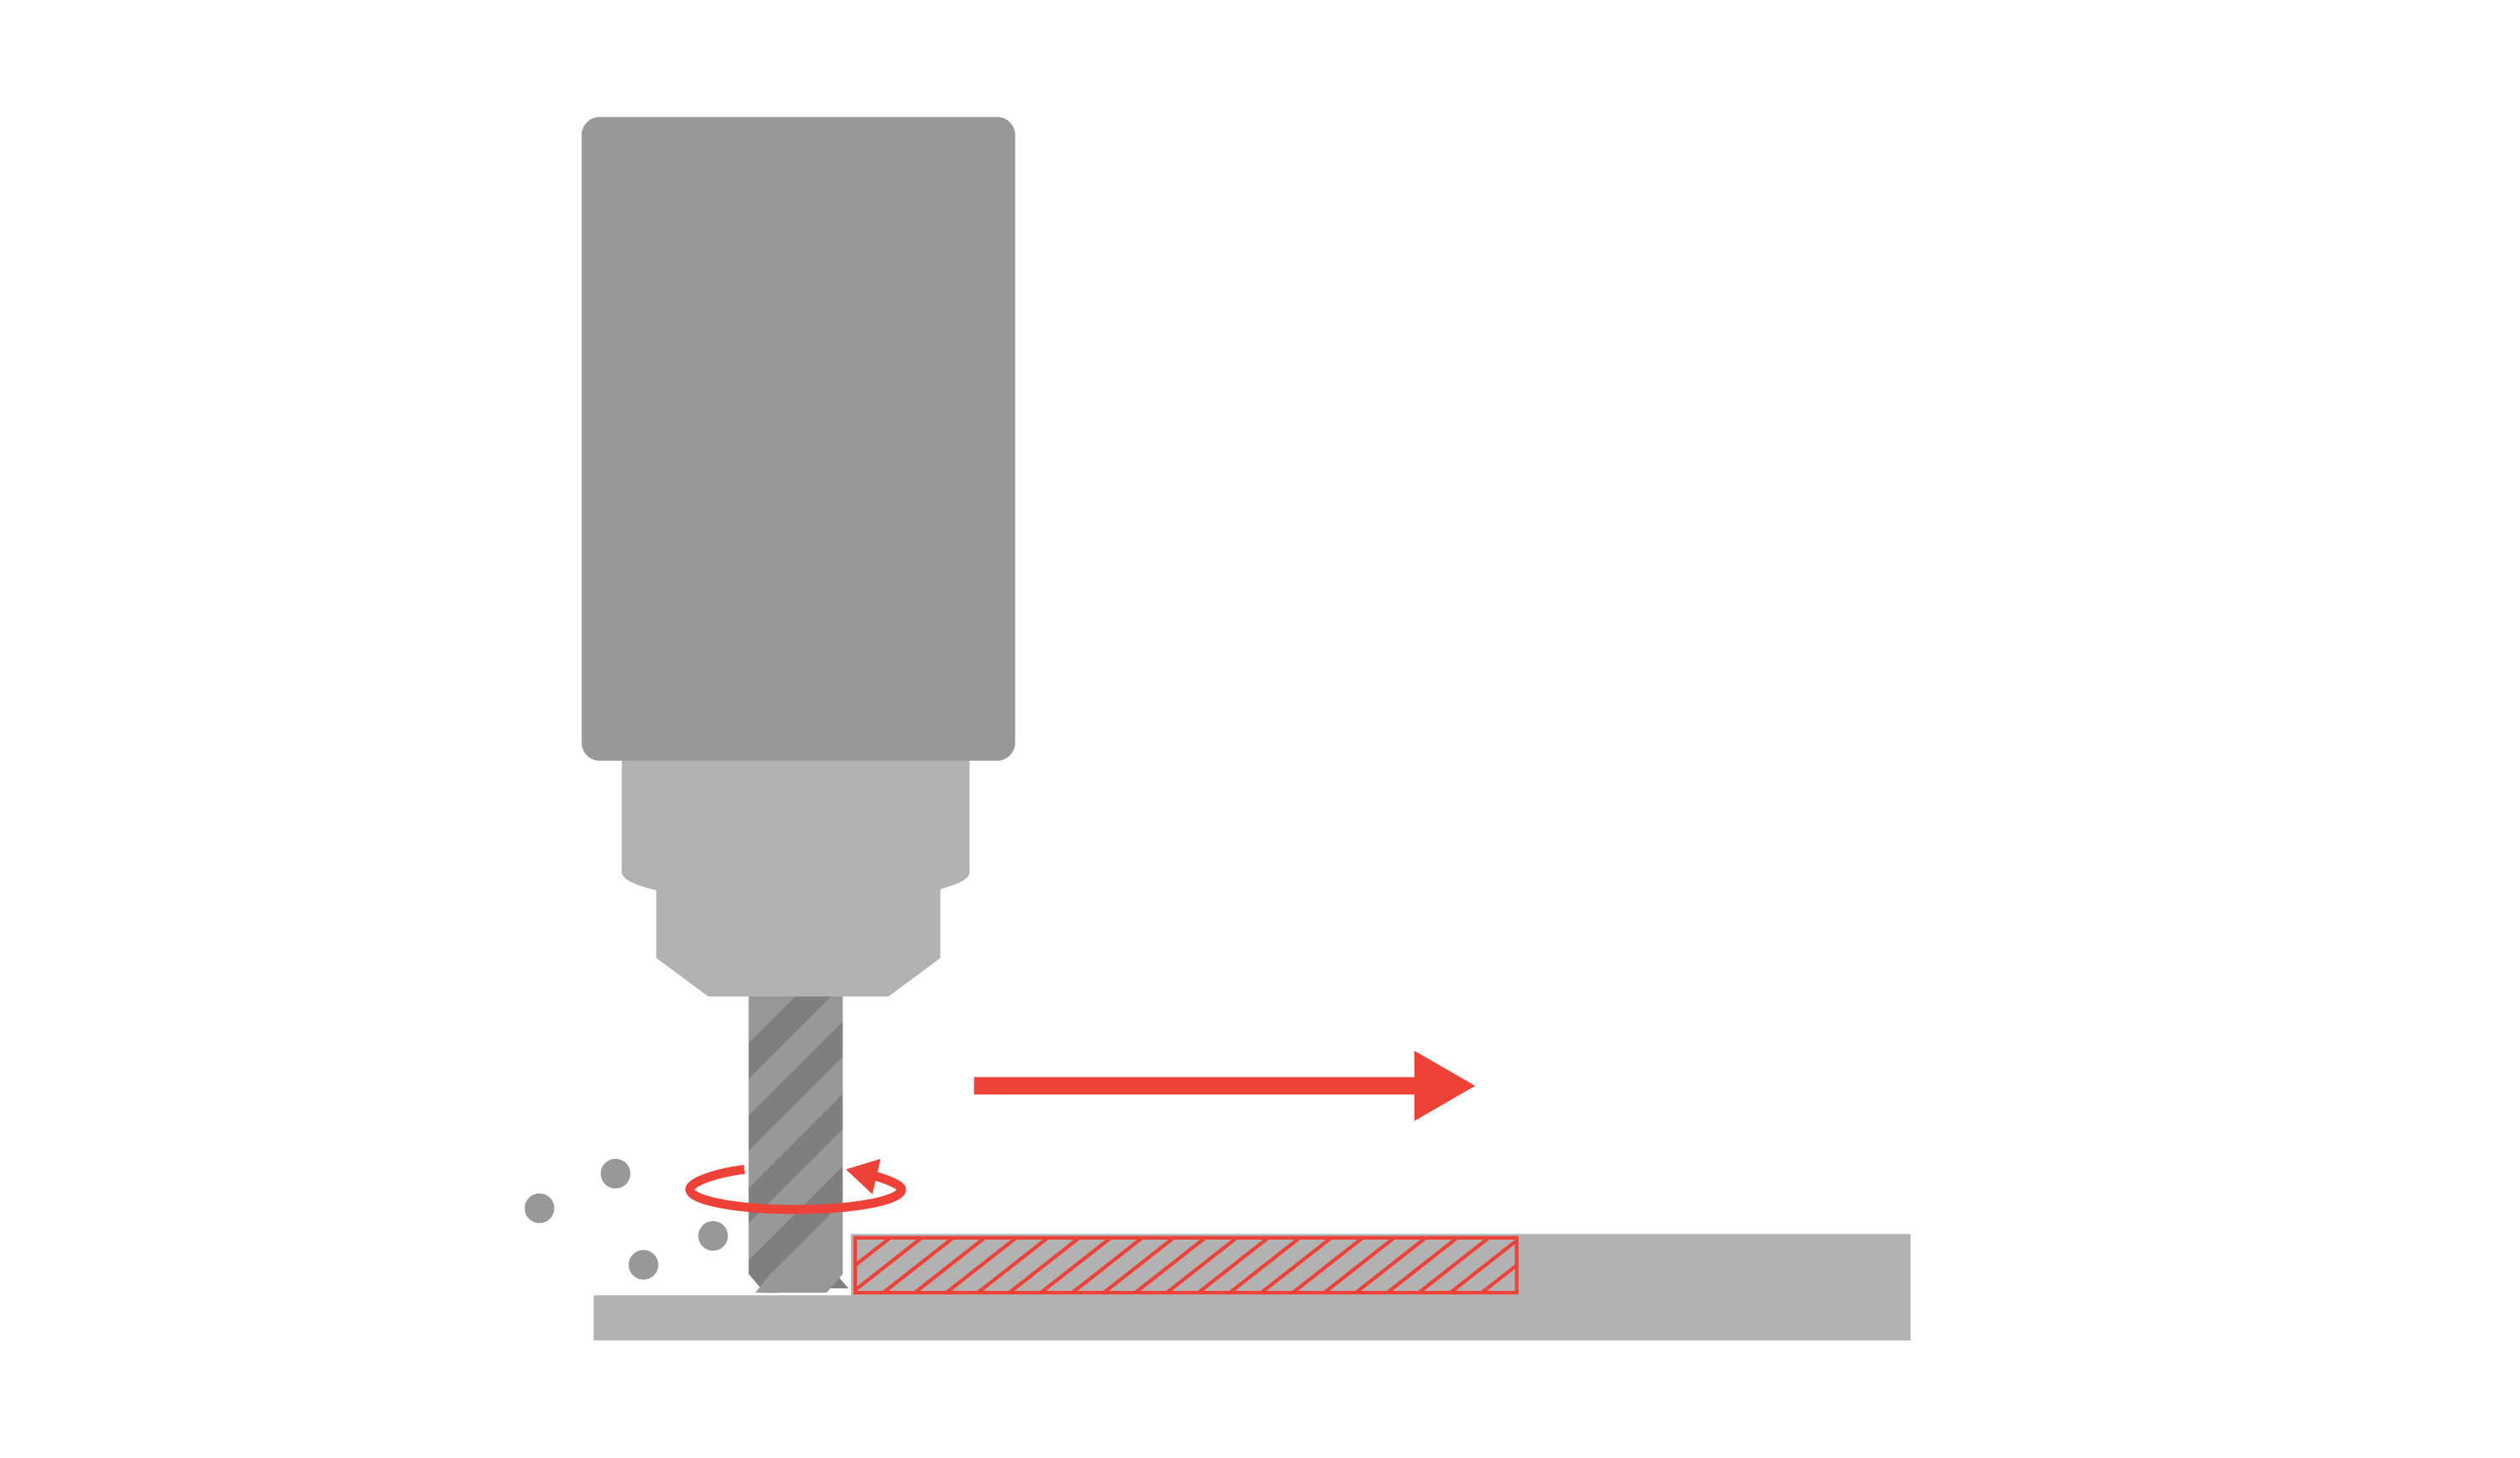
\includegraphics[width=.75\textwidth]{mill1.png}


There are also various different kinds of mills, ranging from a 3-axis mill which can cut out simple shapes in the X, Y, and Z axes, all the way to 6-axis mills that can also rotate about those axes to create more complex curvatures.

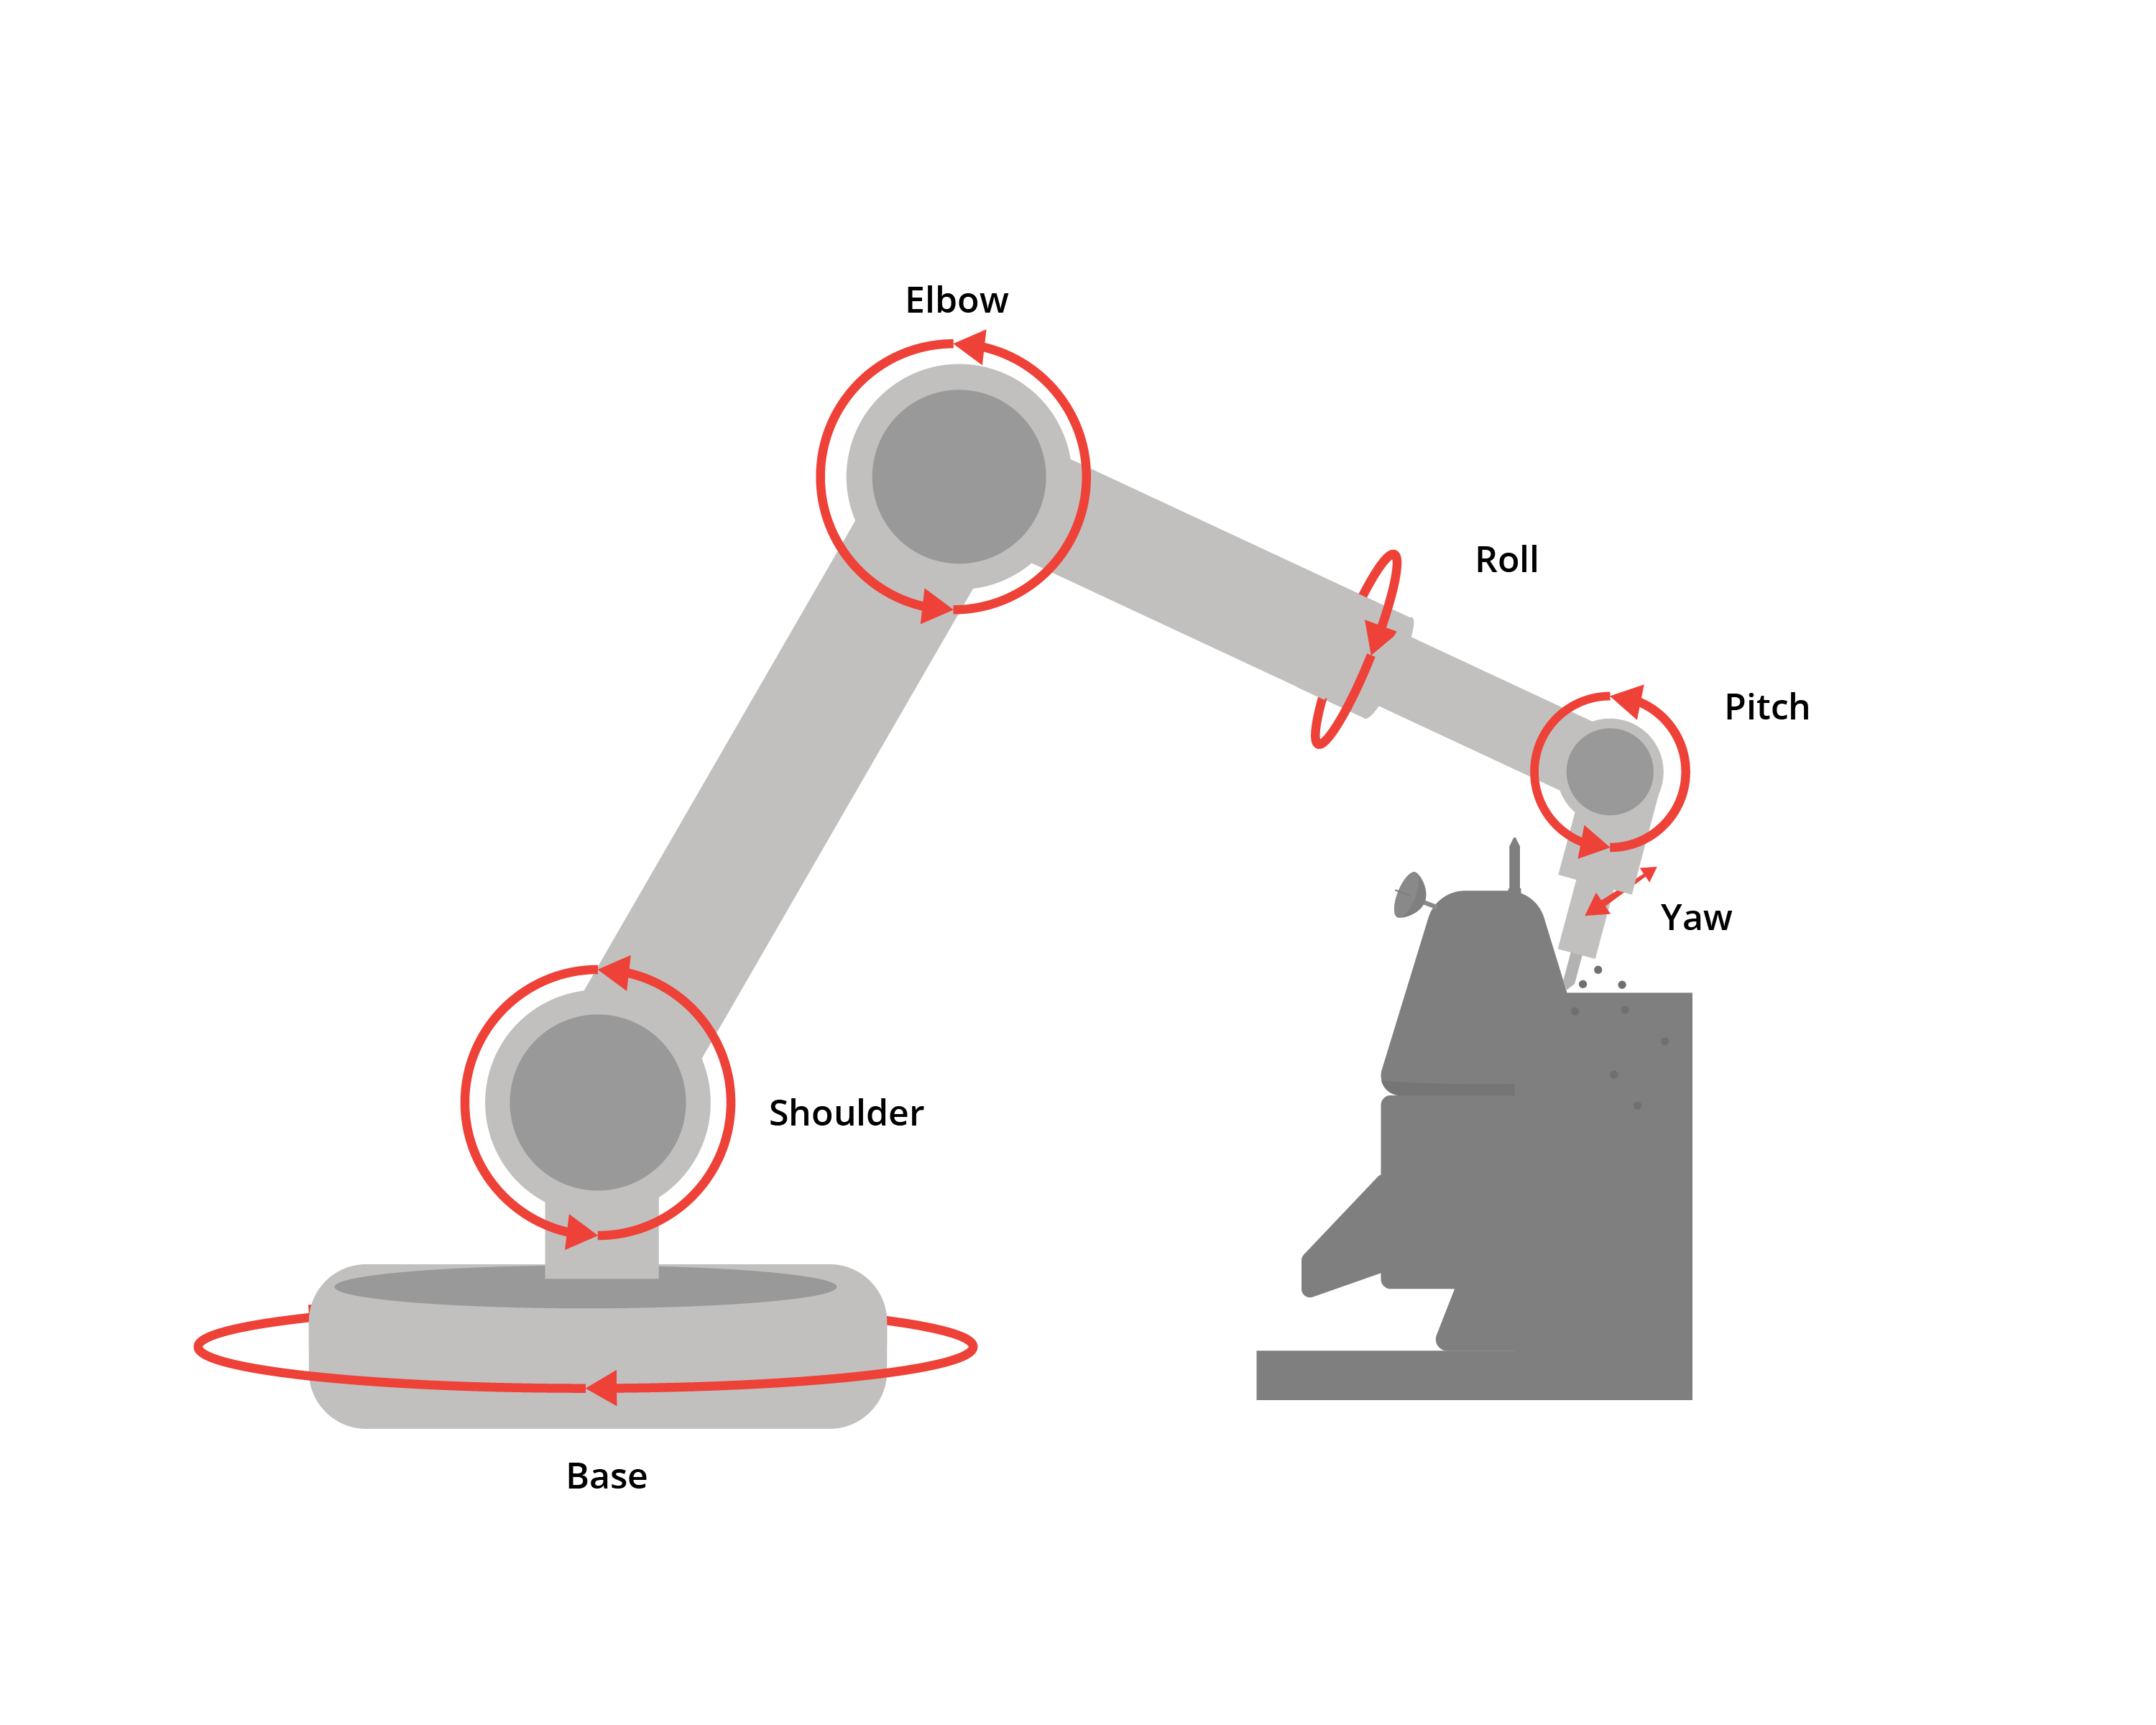
\includegraphics[width=.75\textwidth]{sixAxisCnc.png}


In manufacturing settings where speed and repeatability is paramount, mills are often computer controlled. This functionality is referred to as \newterm{Computer Numerical Control}, or CNC. CNC mills are able to repeatedly follow a tool path, resulting in consistent and accurate parts.

\section{Lathing}

Lathes are tools that allow us to carve out complex cylindrical shapes from raw material. Like a mill it also is a subtractive manufacturing process, however this time it is the material that rotates at a very high speed instead of the tool bit. As the material rotates, the tool bit can be used to extract material layer by layer. 

% graphic showing how a lathe removes material - show cylinder of raw material with rotation arrow indicating it rotates, tool bit and tool path, and lathed result
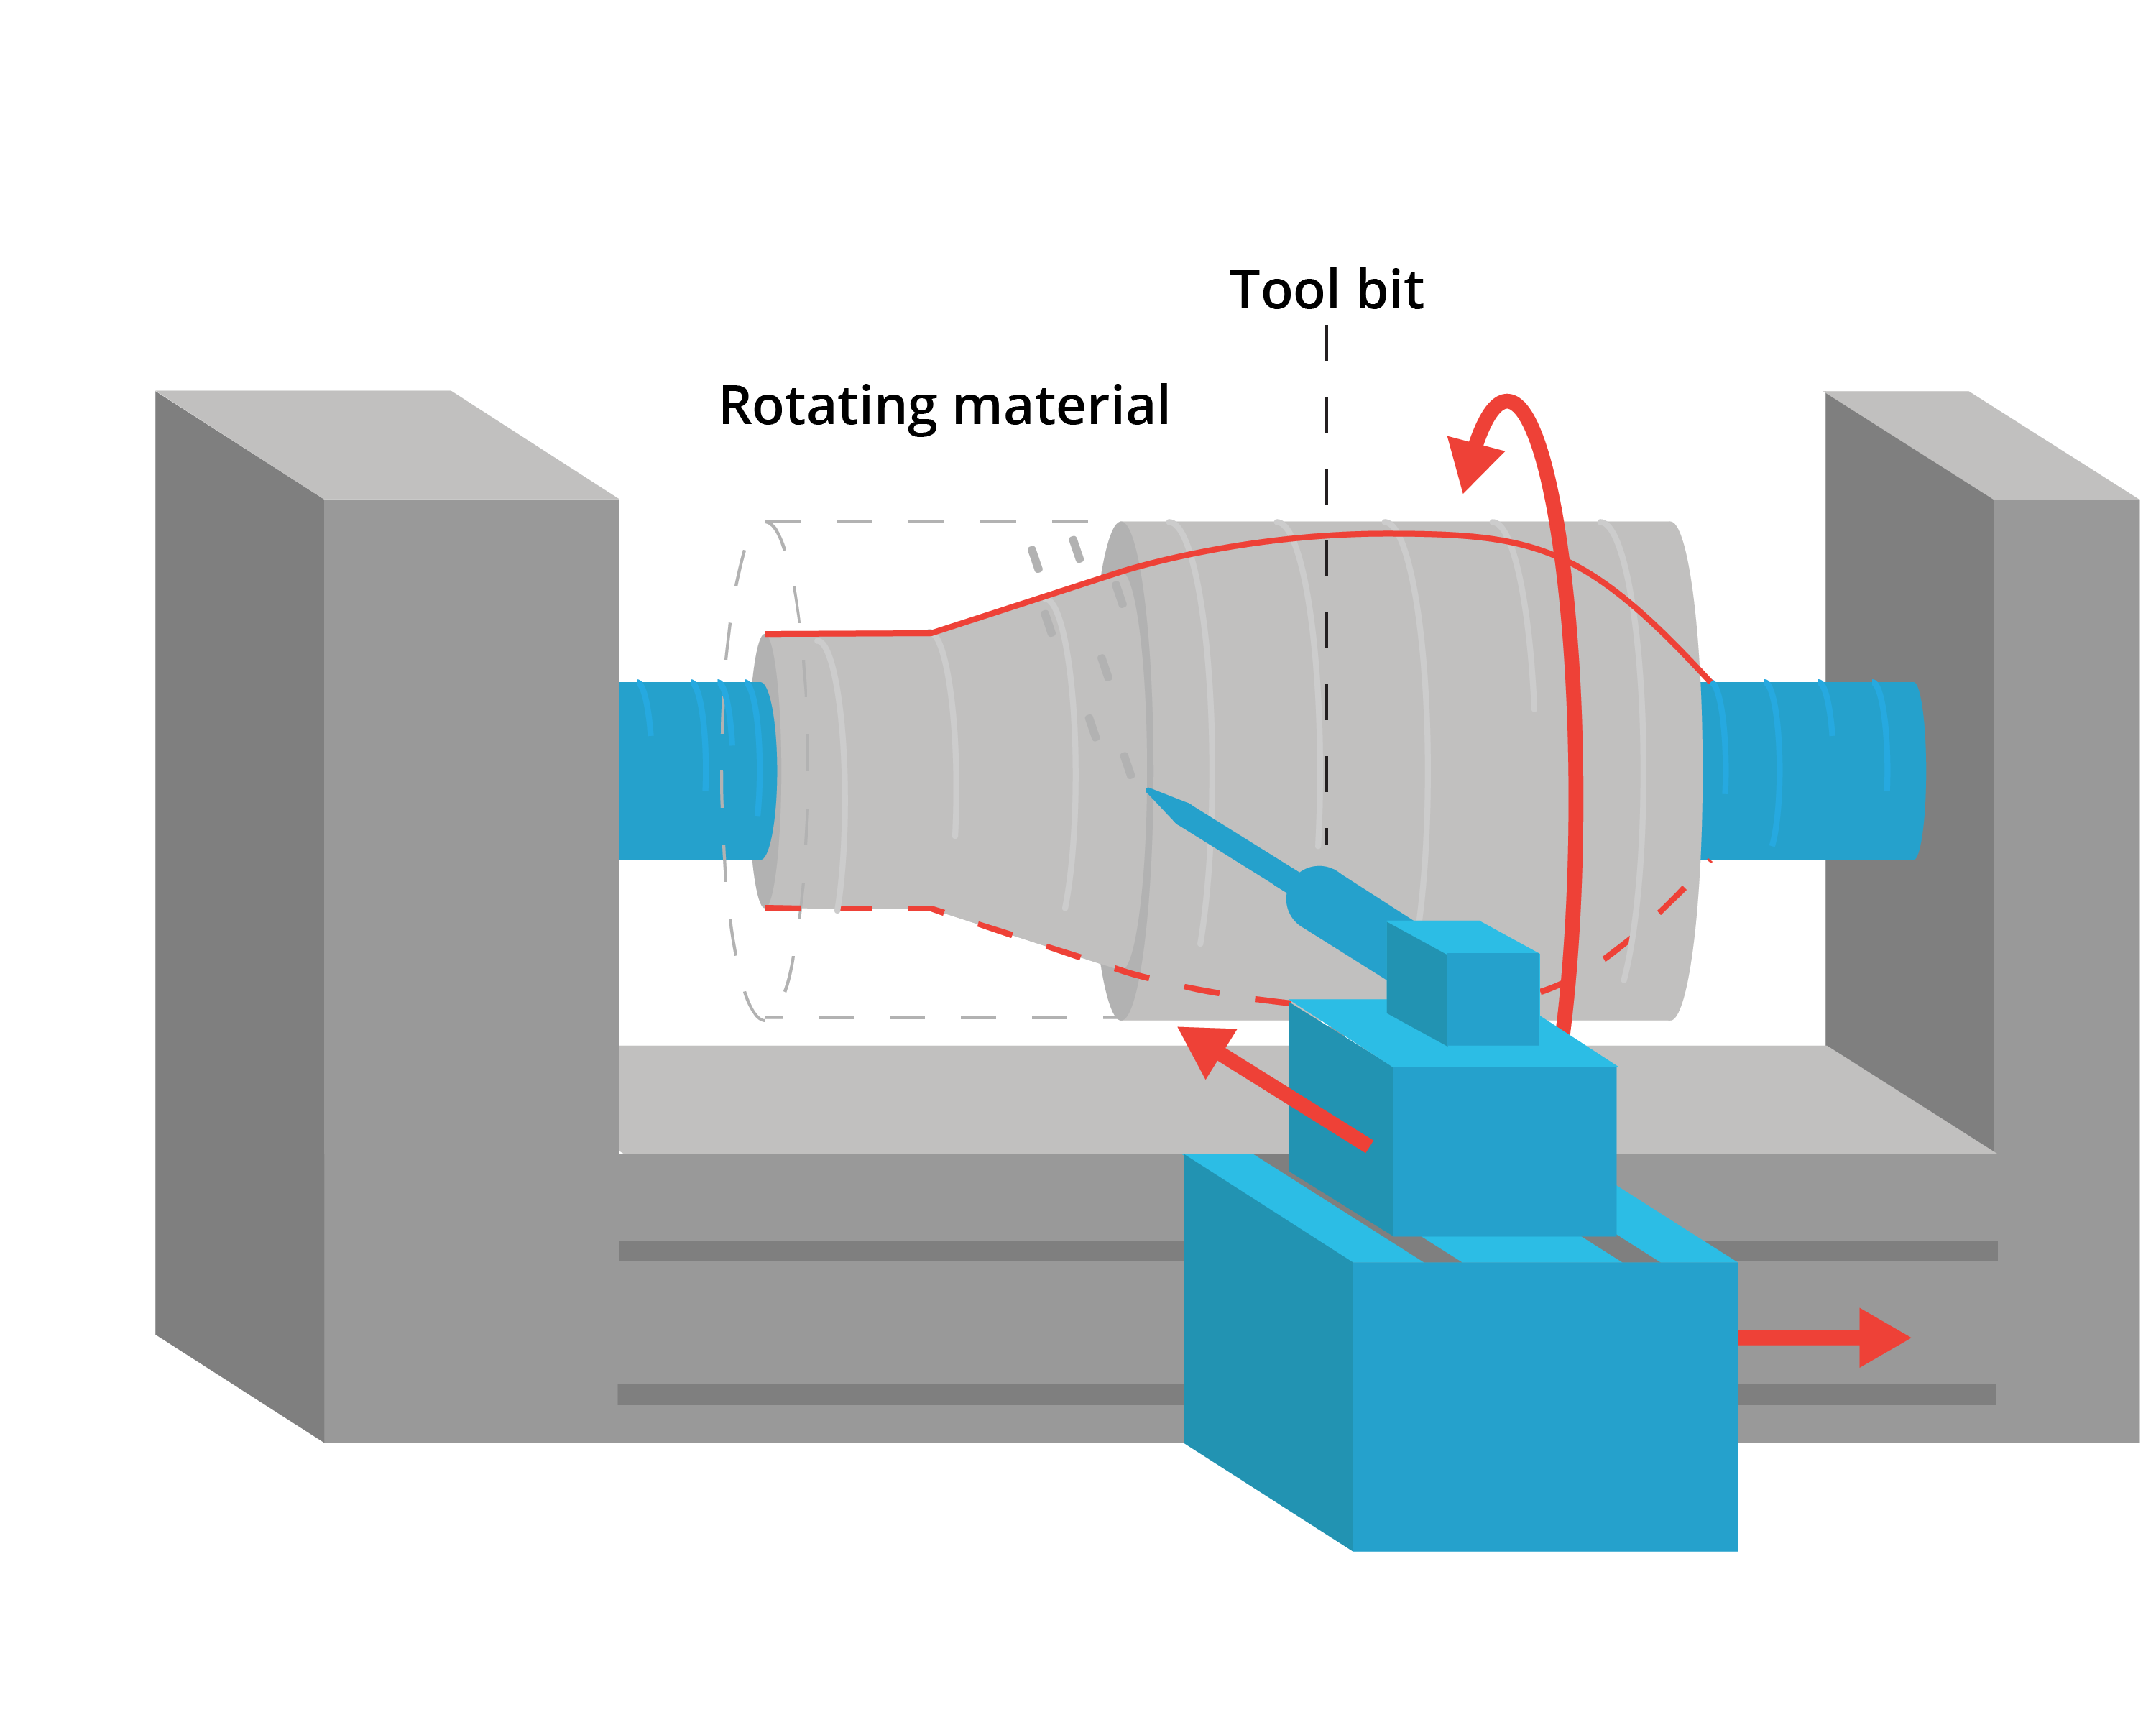
\includegraphics[width=.75\textwidth]{lathe.png}


In the manufacturing industry lathes are also often computer controlled. Along with CNC mills, these CNC lathes are responsible for a majority of the objects that we interact with everyday.

\section{Metal-specific Processes}

While mills and lathes are already able to cover the vast majority of manufacturing needs for woods and metals, there are certain processes that are specifically enabled by the unique properties of metals. More often than not, these processes leverage the malleability of metals at room temperature and at higher temperatures as well.

\section{Sheet Metal Processes}

While milling allows us to process blocks of metal to great effect, sometimes the application we need doesn’t require material of such thickness.

This is where sheet metal comes in, and the methods we use to process it. One of the most common in manufacturing is rolling, where a raw sheet is gradually rolled into the desired shape. This method is used to create many objects you may recognize, such as metal roofings, aircraft frames, and more.

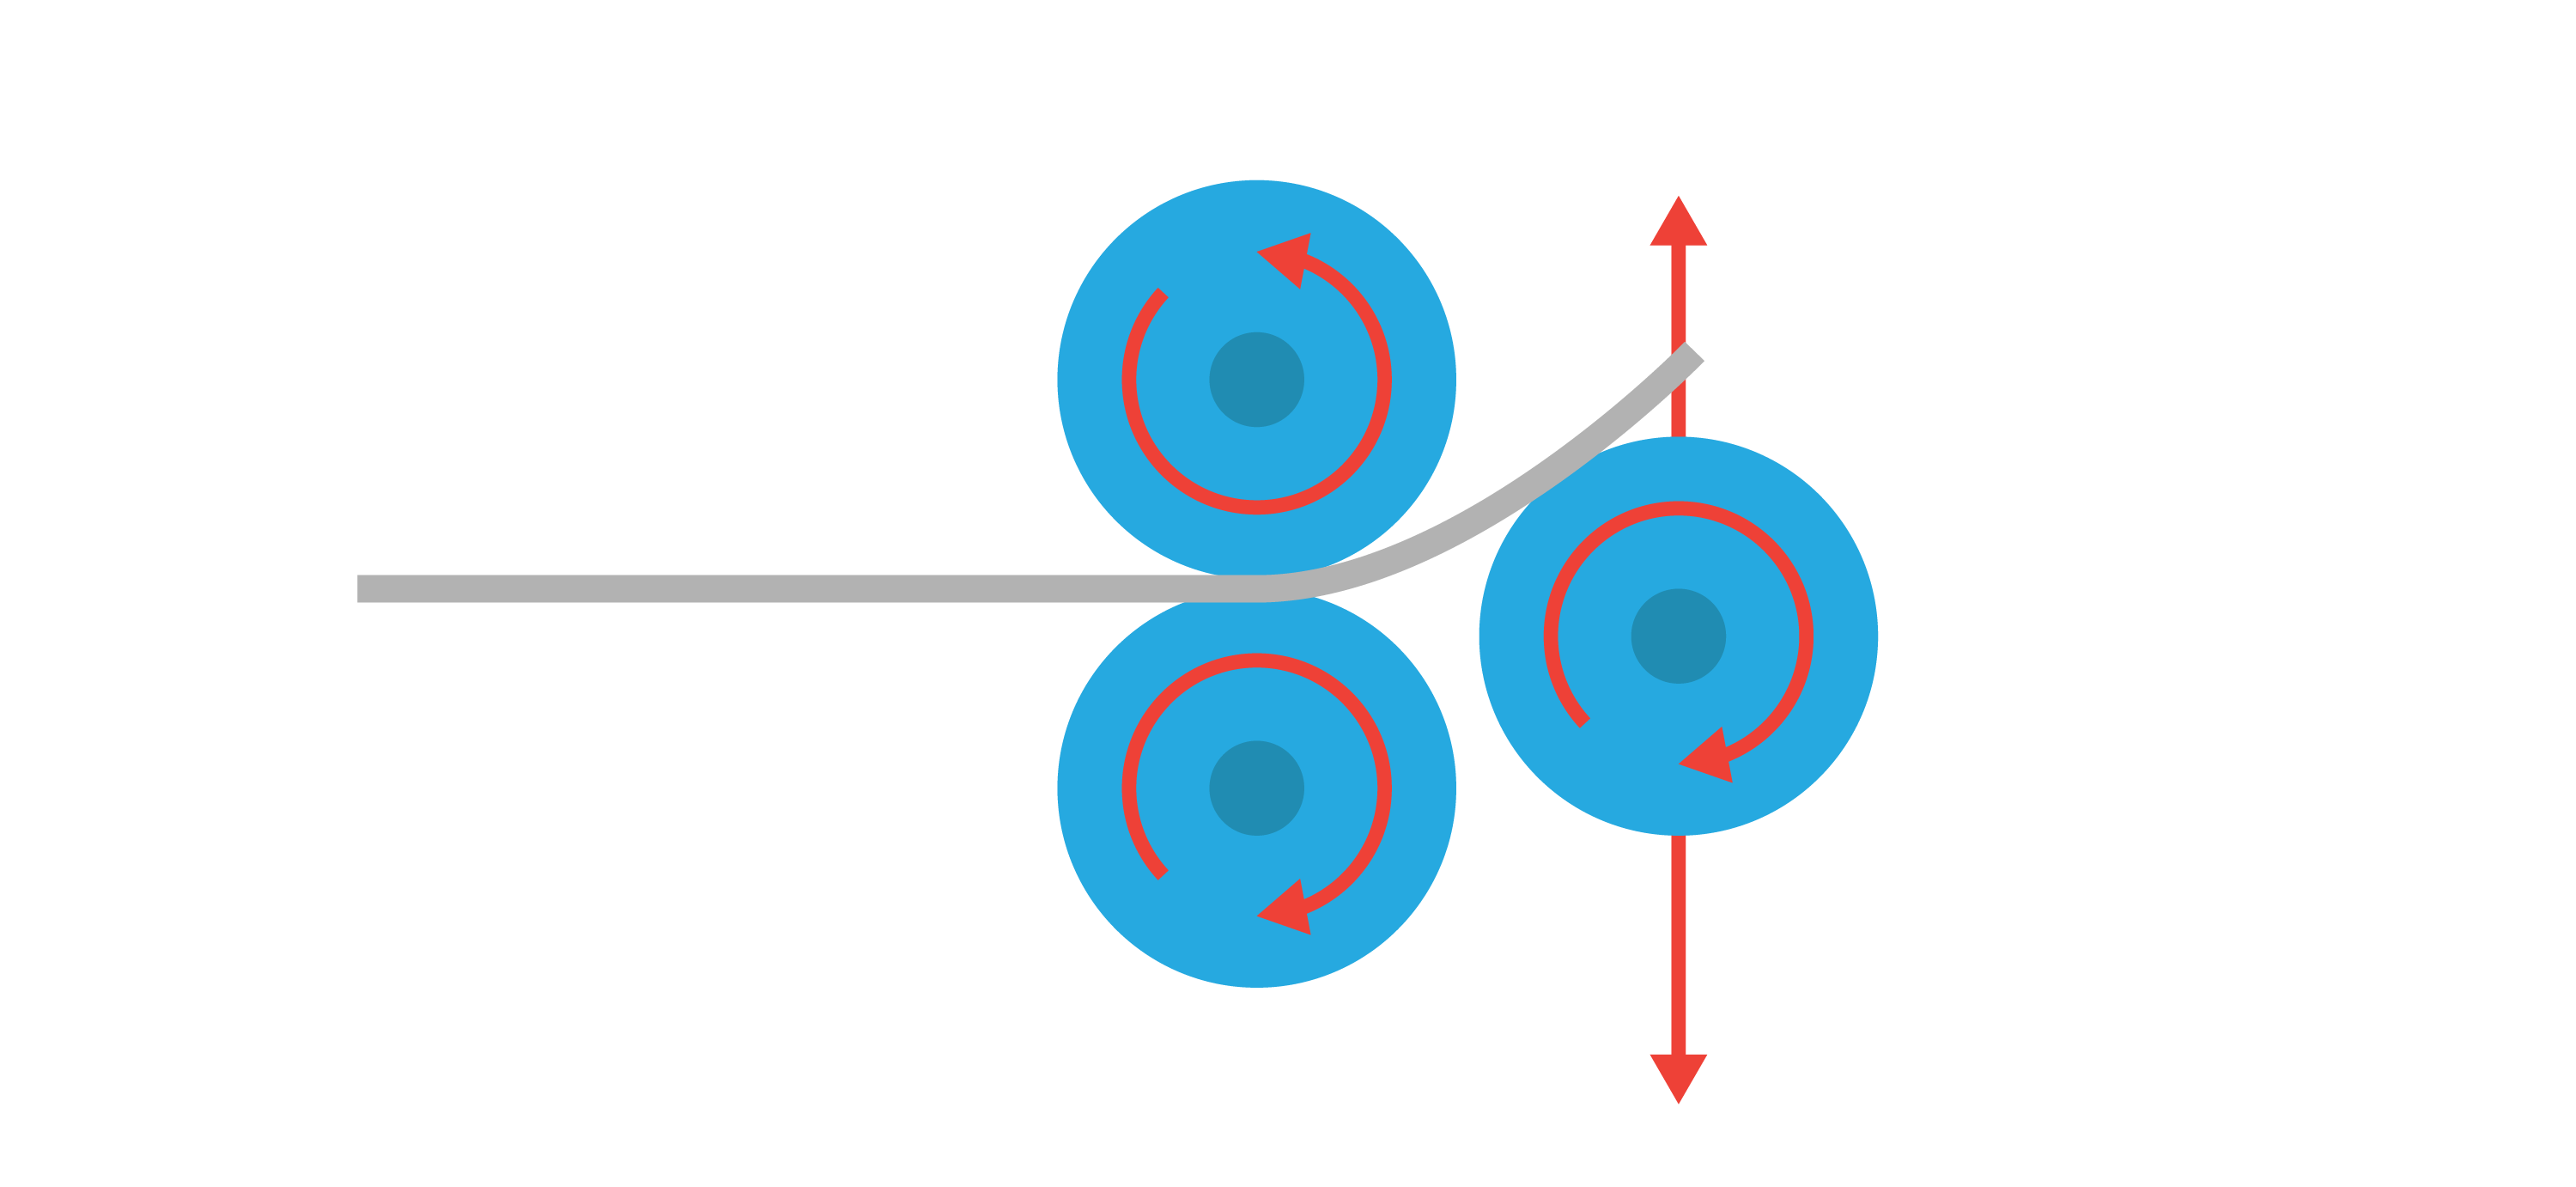
\includegraphics[width=.75\textwidth]{rolling.png}


Another method is stamping, where a raw sheet is stamped into the desired shape. This allows us to create surfaces with complex geometries in an instant, and in large quantities. This method is often used for applications such as the exterior panels of a car, where parts with compound curves are needed.

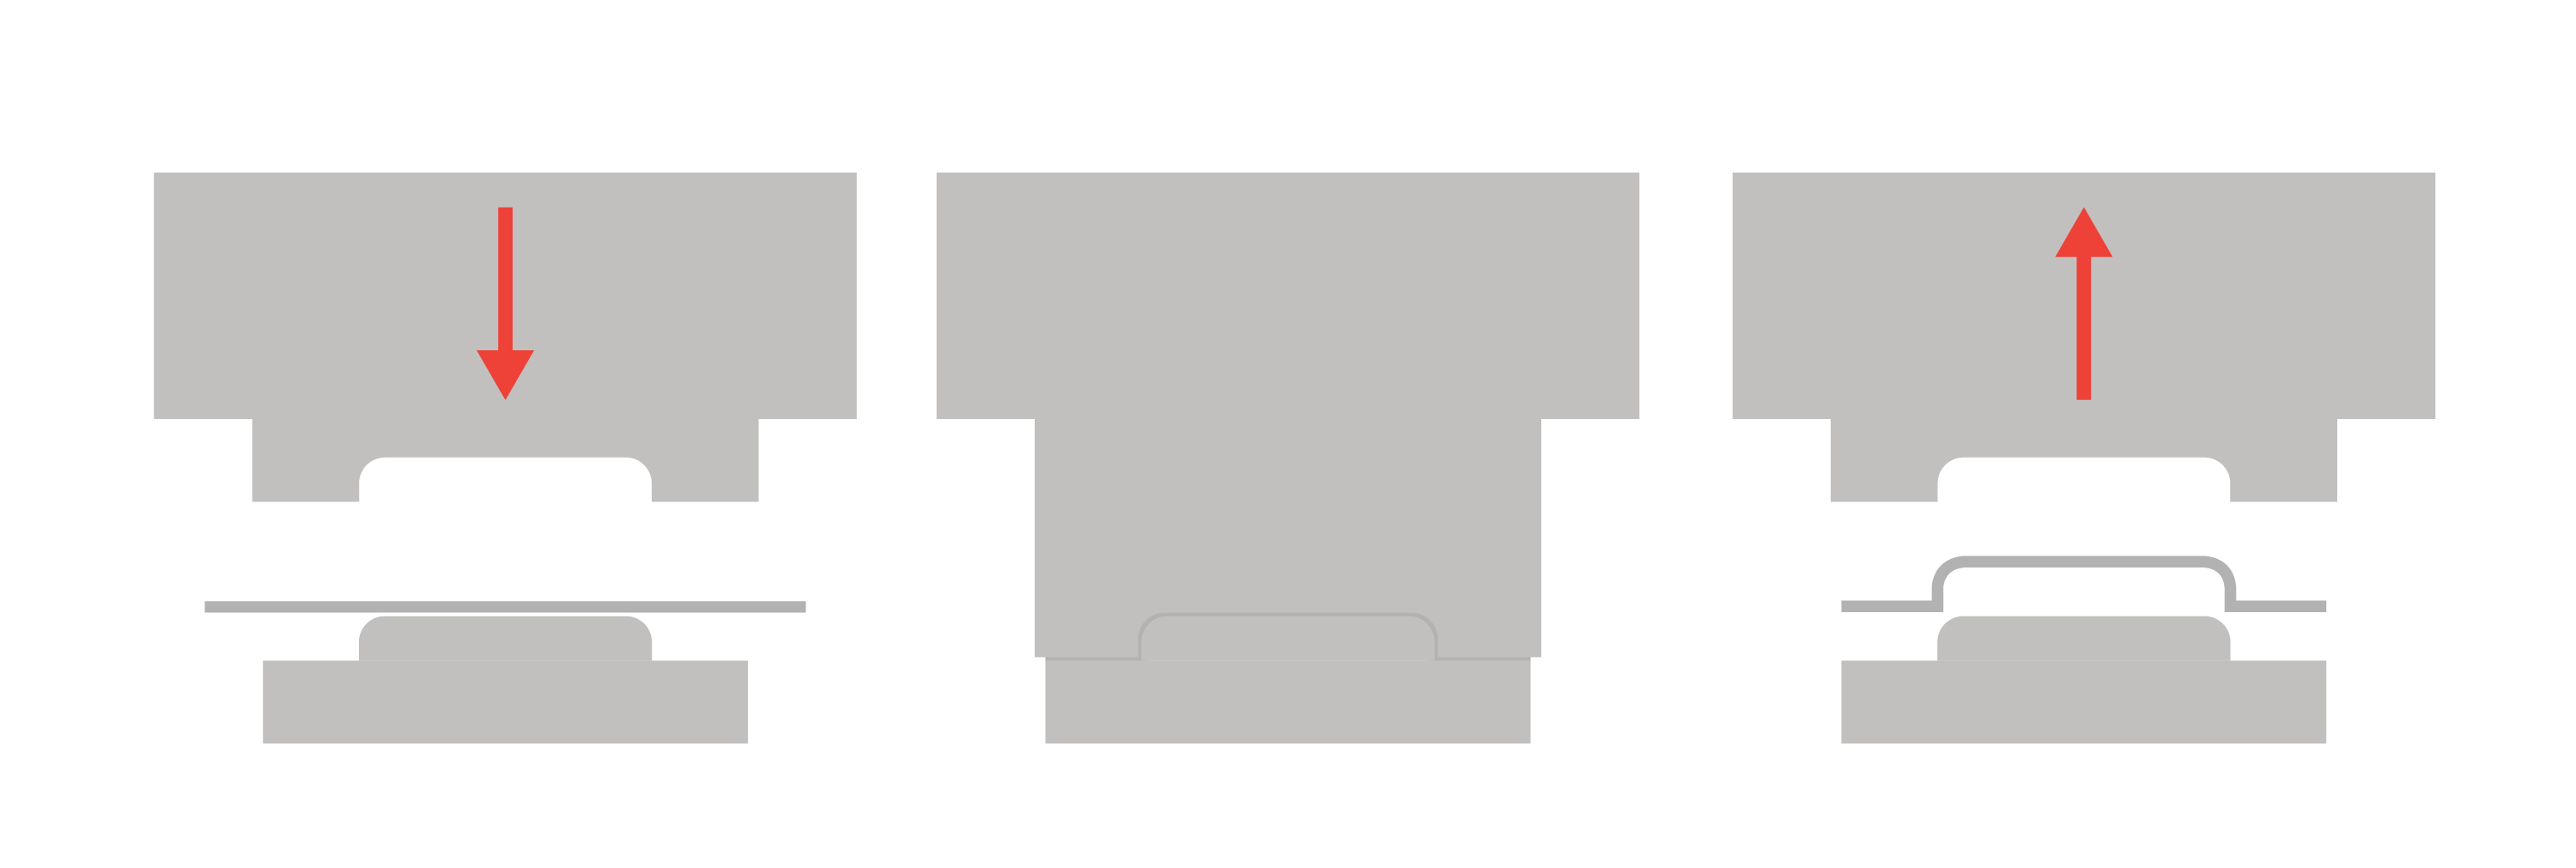
\includegraphics[width=.75\textwidth]{stamping.png}


%graphic of a flat sheet stamped into a car door shape e.g.

Lastly, there are also separate processes used to increase the strength of sheet metal parts. This falls under the category of sheet metal forming, and involves bending the edges of a part to form a reinforced flap. Almost all sheet metal parts are reinforced in this manner, as it is a relatively simple process and also helps to create a clean edge for a more finished look.

\section{Casting}

The last kind of metal-specific process we’ll cover is casting. Casting involves pouring molten metal into a mold, and then letting the metal cool and set inside the mold. Smaller components with complex geometries and limited structural requirements such as toys are often cast, as it is an accurate and high-volume manufacturing method.

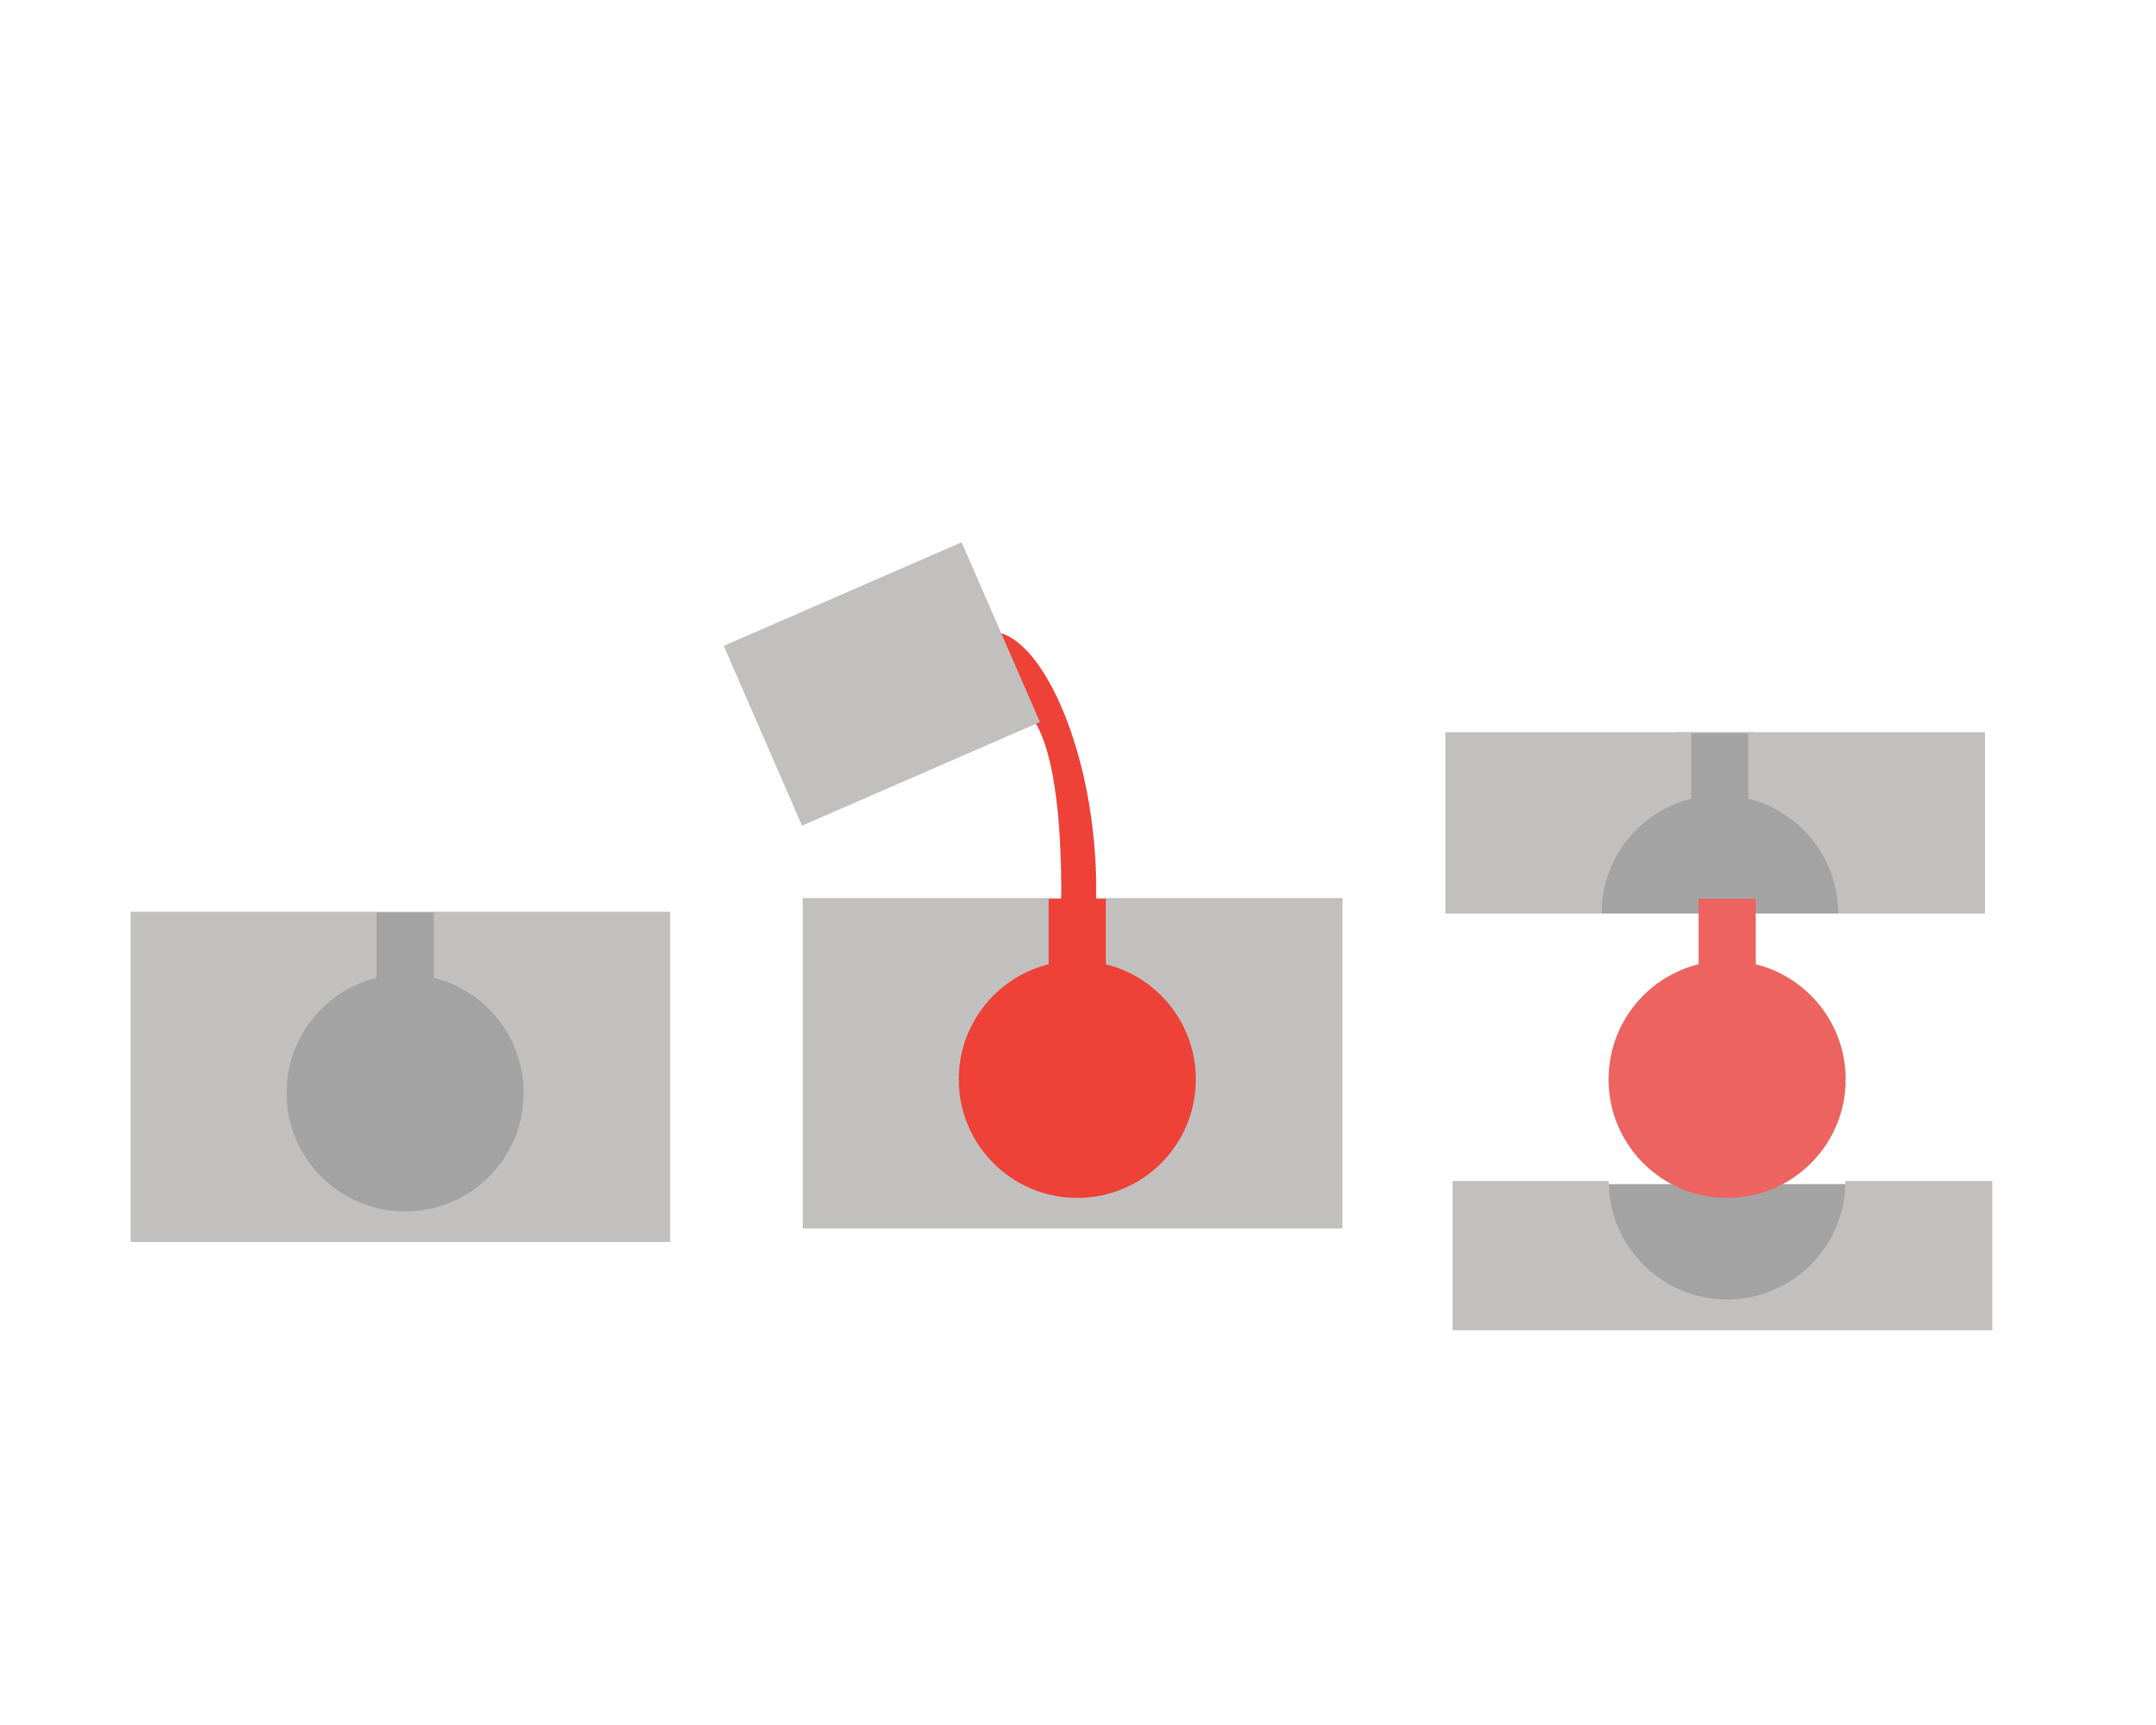
\includegraphics[width=.75\textwidth]{casting.png}


Casting also results in minimal material wastage, as it is not a subtractive manufacturing method where excess material is machined away, but rather only the specific amount of material required is poured in each time.

\section{Wood-specific Processes}

Similar to metals, there are also certain manufacturing processes that are enabled by the unique qualities of wood. These make use of the water content inherent in wood, and the flexibility it enables.

\section{Bending}

Turning raw wood into flat, workable pieces involves a variety of tools that you probably know of already, such as saws and drills. But there are specific processes that help us create curved shapes with wood, besides the mill and the lathe mentioned earlier.

This is where bent lamination comes in. Bent lamination involves layering multiple thin veneers or strips of wood with adhesive, and clamping it to create the desired form while letting the glue dry. This method is often used for furniture production, enabling continuous curves in wood with tight radii.

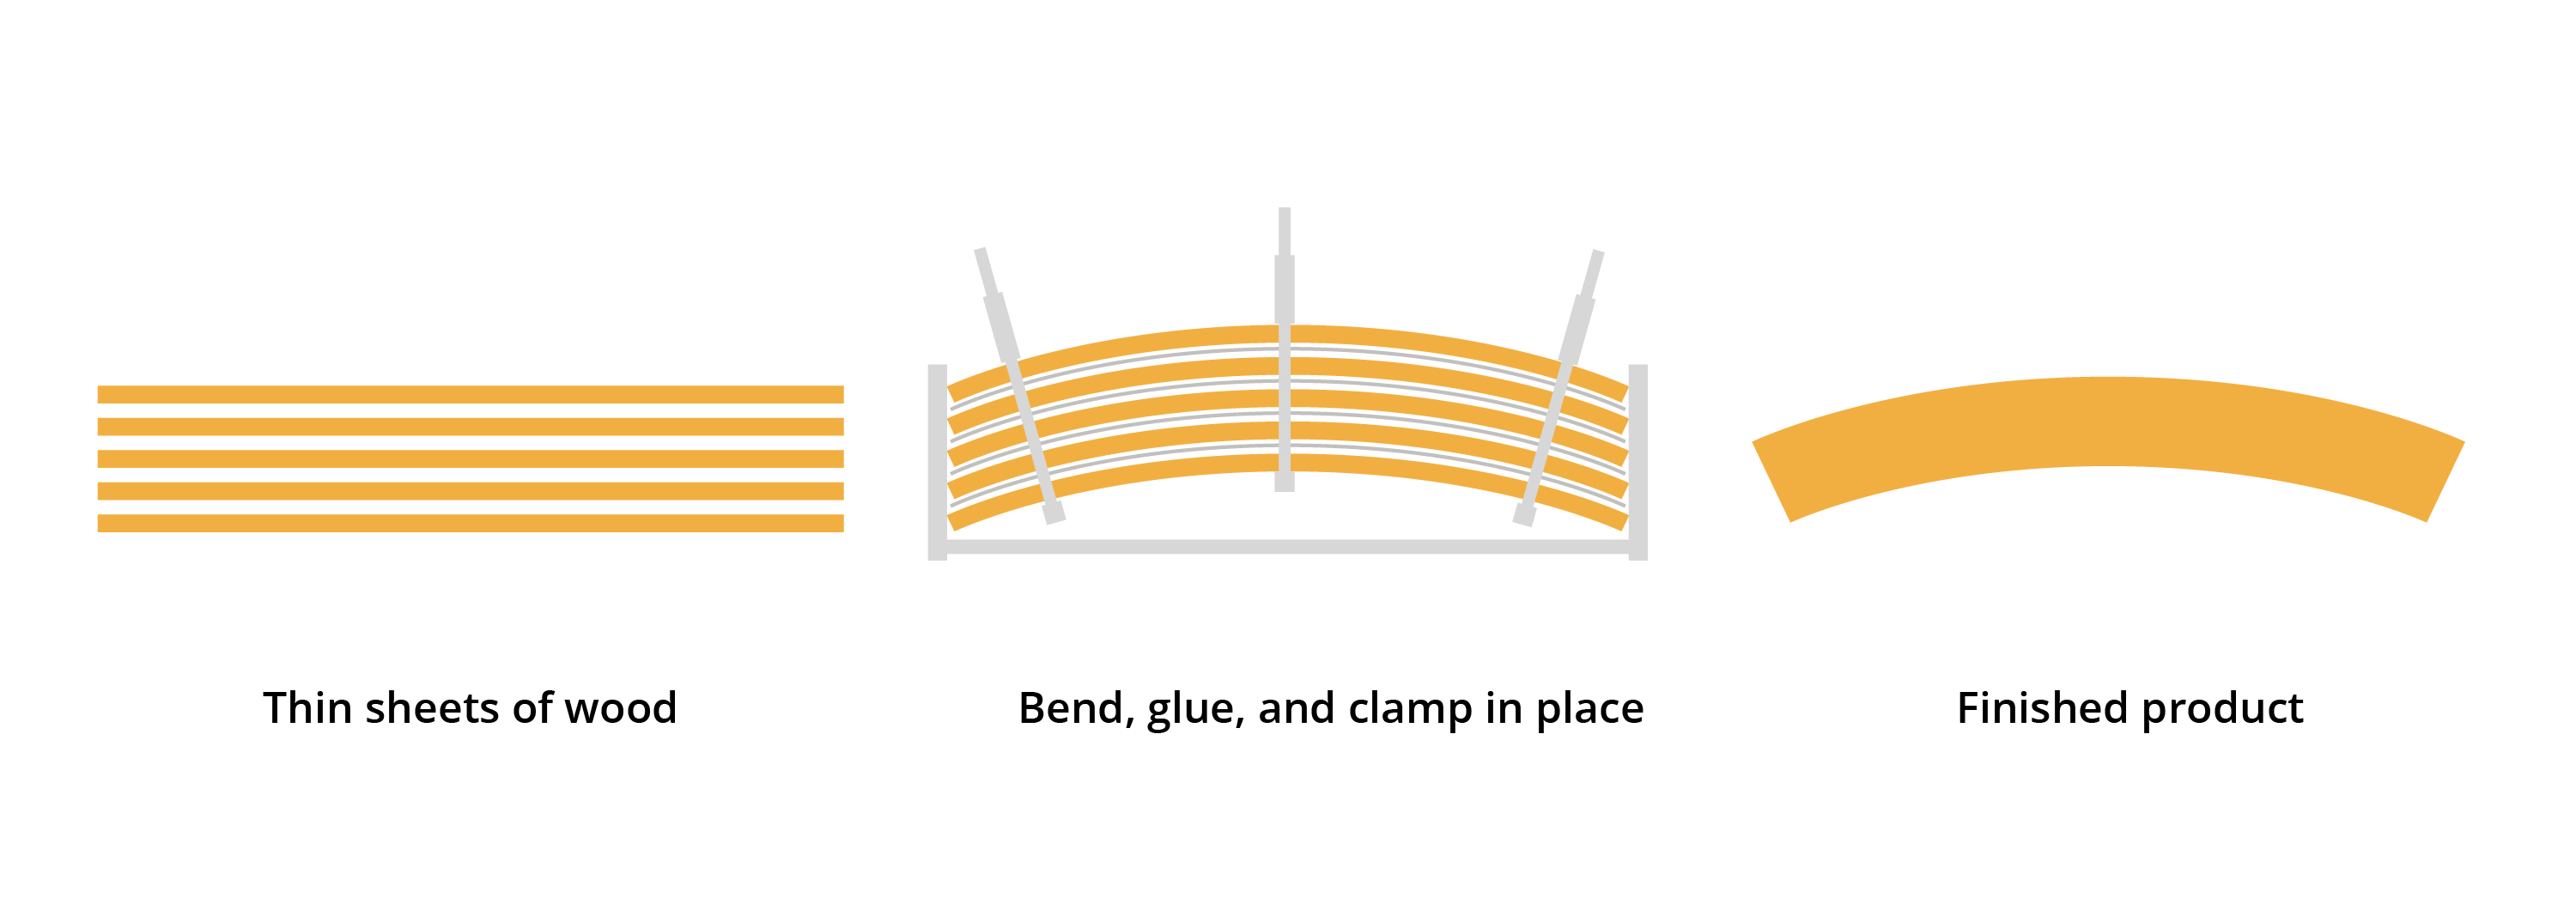
\includegraphics[width=.75\textwidth]{woodBend.png}

%graphic of bent lamination - various veneers being layered, then clamped within a form, and then the final result

Steam can also be used for bending, by helping soften the wood fibers to increase flexibility. Once the desired form is reached, the part can then cool down and harden. Unlike bent lamination, steam bending can be done without adhesives.

\section{Plastic-specific Processes}

Although plastics only came into prominence in the mid 20th century, they have changed manufacturing and by extension the world as we know it. Easily manufacturable, durable, and cost-effective, they’ve come to permeate almost everything we use on a daily basis.

It must also be noted that these exact qualities have also resulted in the proliferation of plastics in our environment, and as such usage of plastics should be well considered and limited. Alternative biodegradable materials are currently being trialled by scientists and would look to replicate many of the same qualities we expect from plastics, including its manufacturability.

\section{Injection Molding}

Injection molding is responsible for the vast majority of plastic products that you interact with on a daily basis. It’s extremely quick, highly accurate, and has minimal material wastage, making it a popular and cost effective method of manufacturing plastic goods.

Similar to casting, injection molding involves injecting molten plastic into a mold, and then allowing the part to cool and set inside the cavity. 

You can often tell when a part was produced through injection molding, with telltale signs such as the parting line. This is where the parts of the mold meet, forming a visible line on the surface of a part.

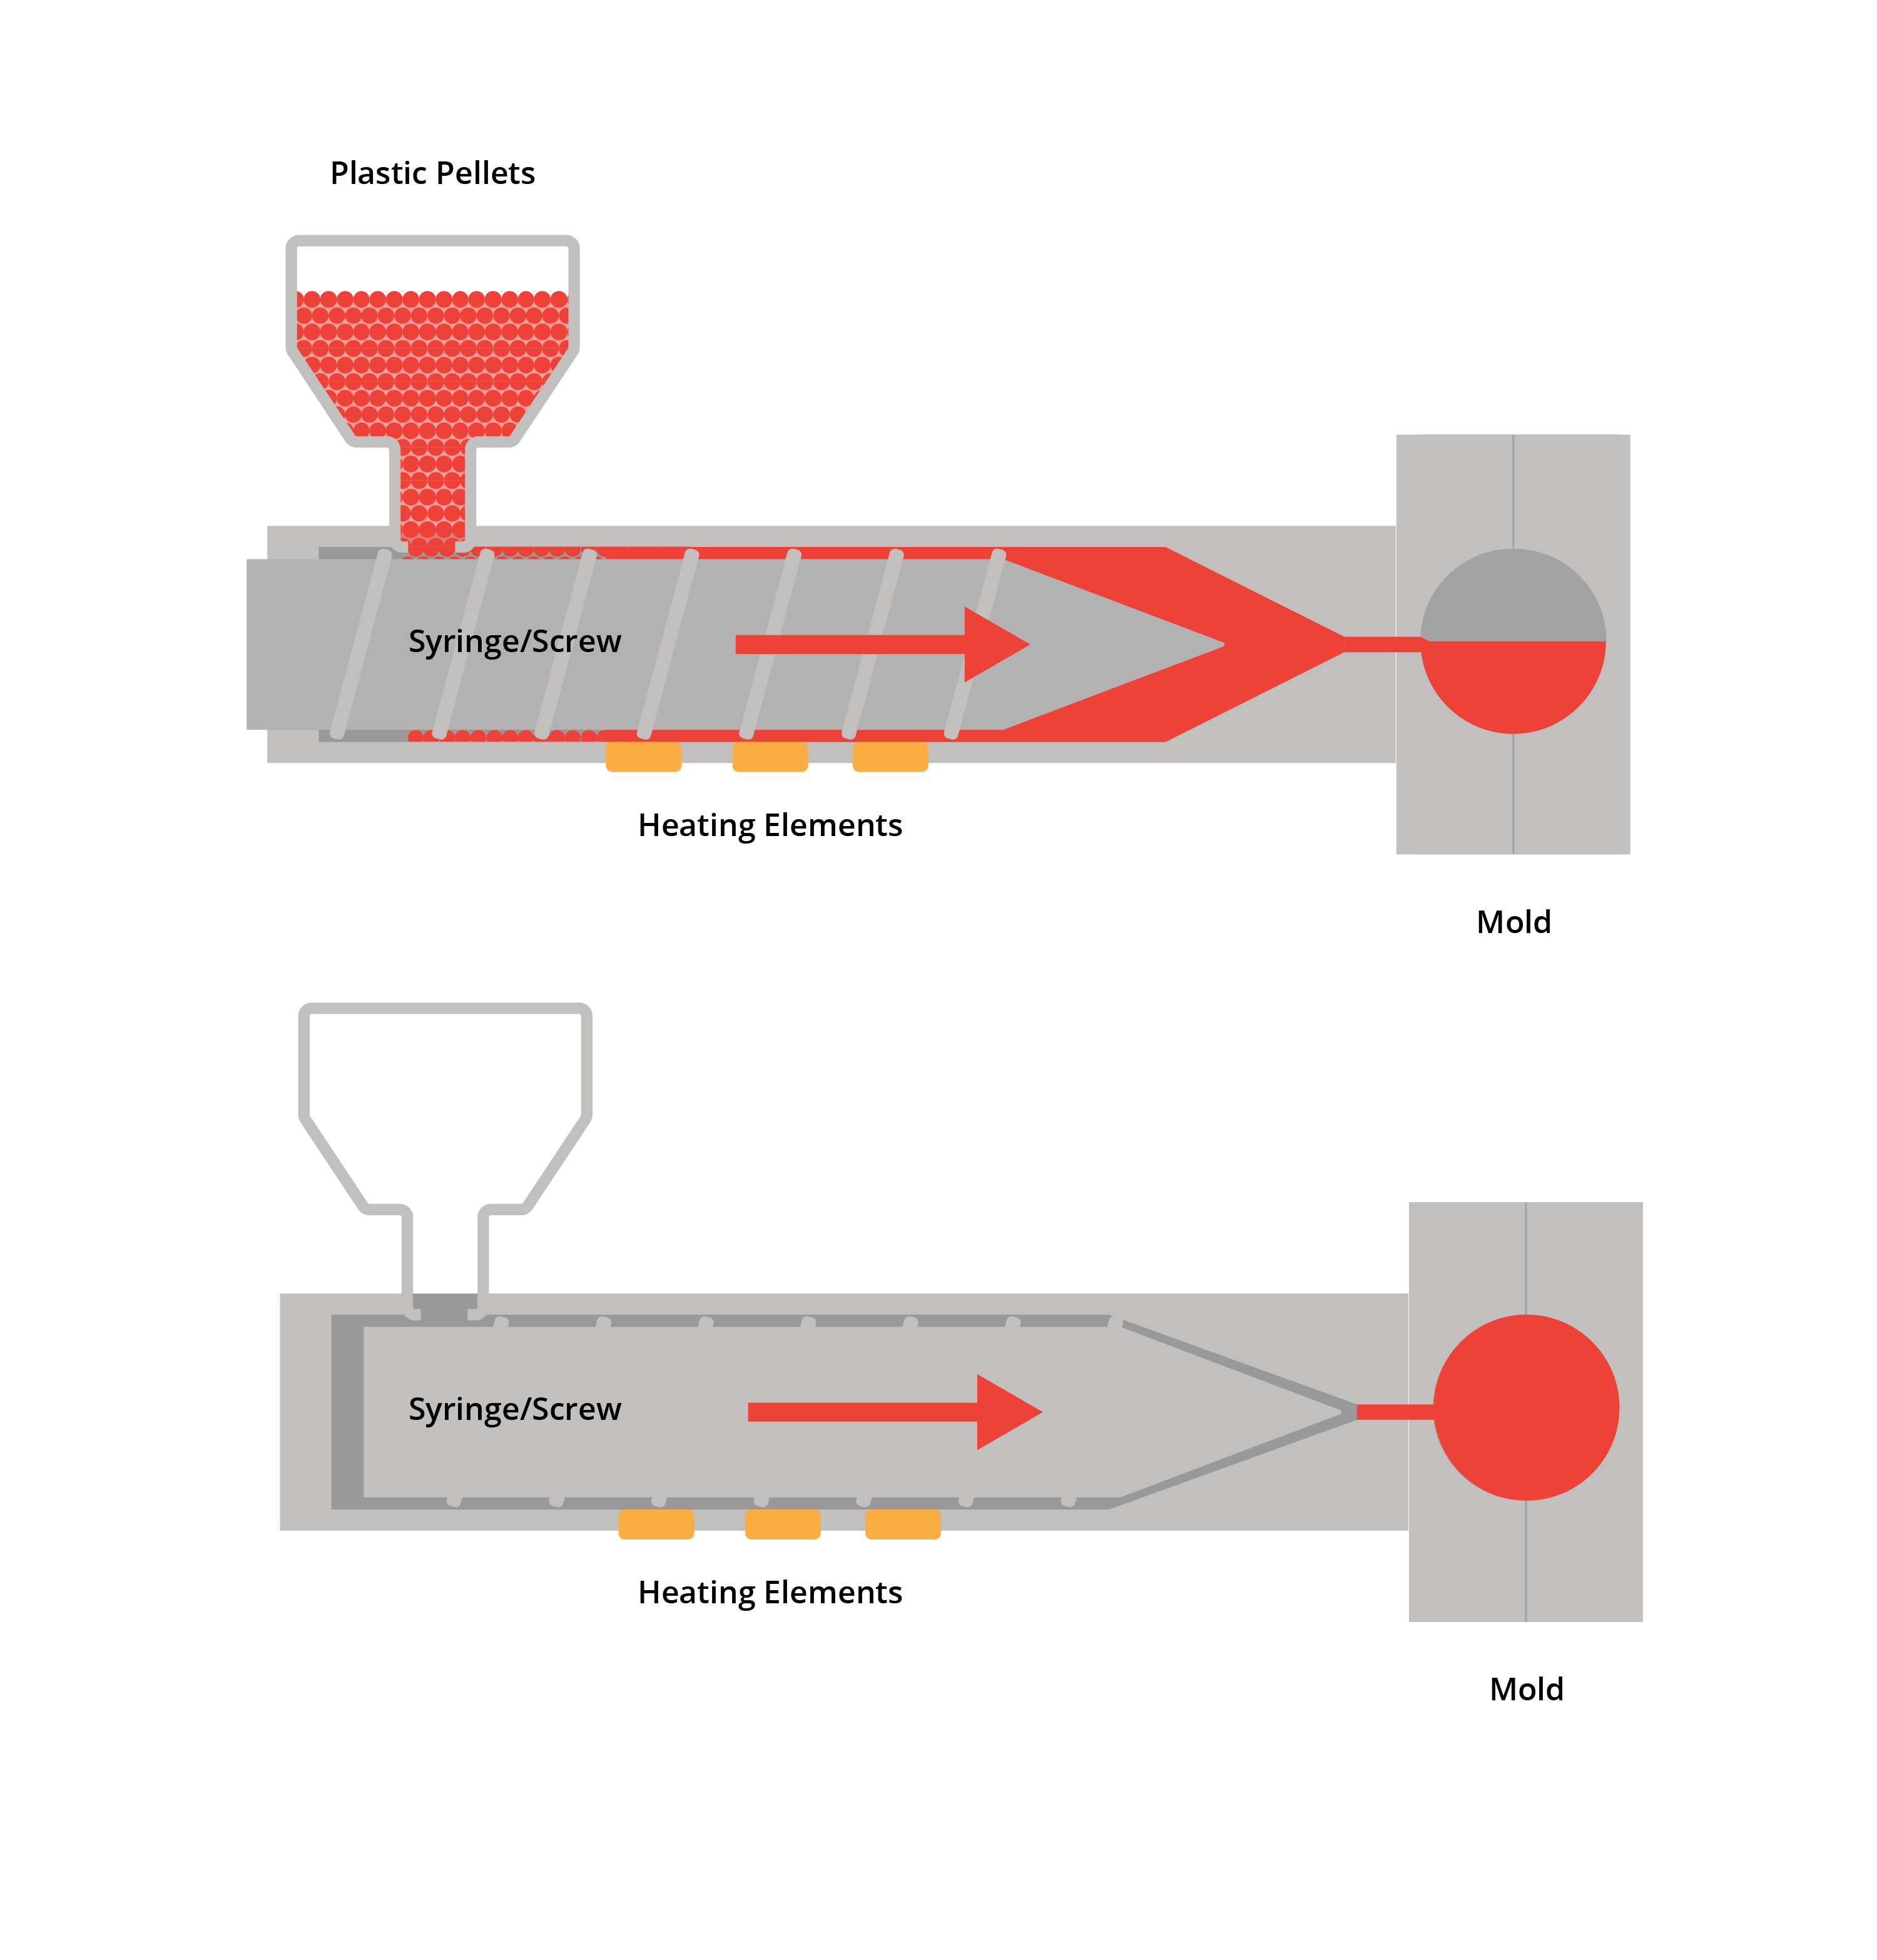
\includegraphics[width=.75\textwidth]{injectionMolding.png}


%graphic showing injection molding with a two part mold - pellets forced into a two part mold, mold closing, and then mold opened with the newly made part (draw a light parting line on the part)

\section{3D Printing}

Injection molding has traditionally been the go-to technique for manufacturing plastic goods, however new technologies result in the advent of new manufacturing methods. 3D printing is one of them, having come to prominence in the last few decades as a way to quickly prototype parts without having to create the molds needed for injection molding.

3D printing is an \newterm{additive} manufacturing process, where molten material is applied layer by layer to form the desired geometry. It allows for complex geometries, and whilst the accuracy may currently lag behind traditional injection molding, it is also improving rapidly.

%graphic for illustrating 3D printing
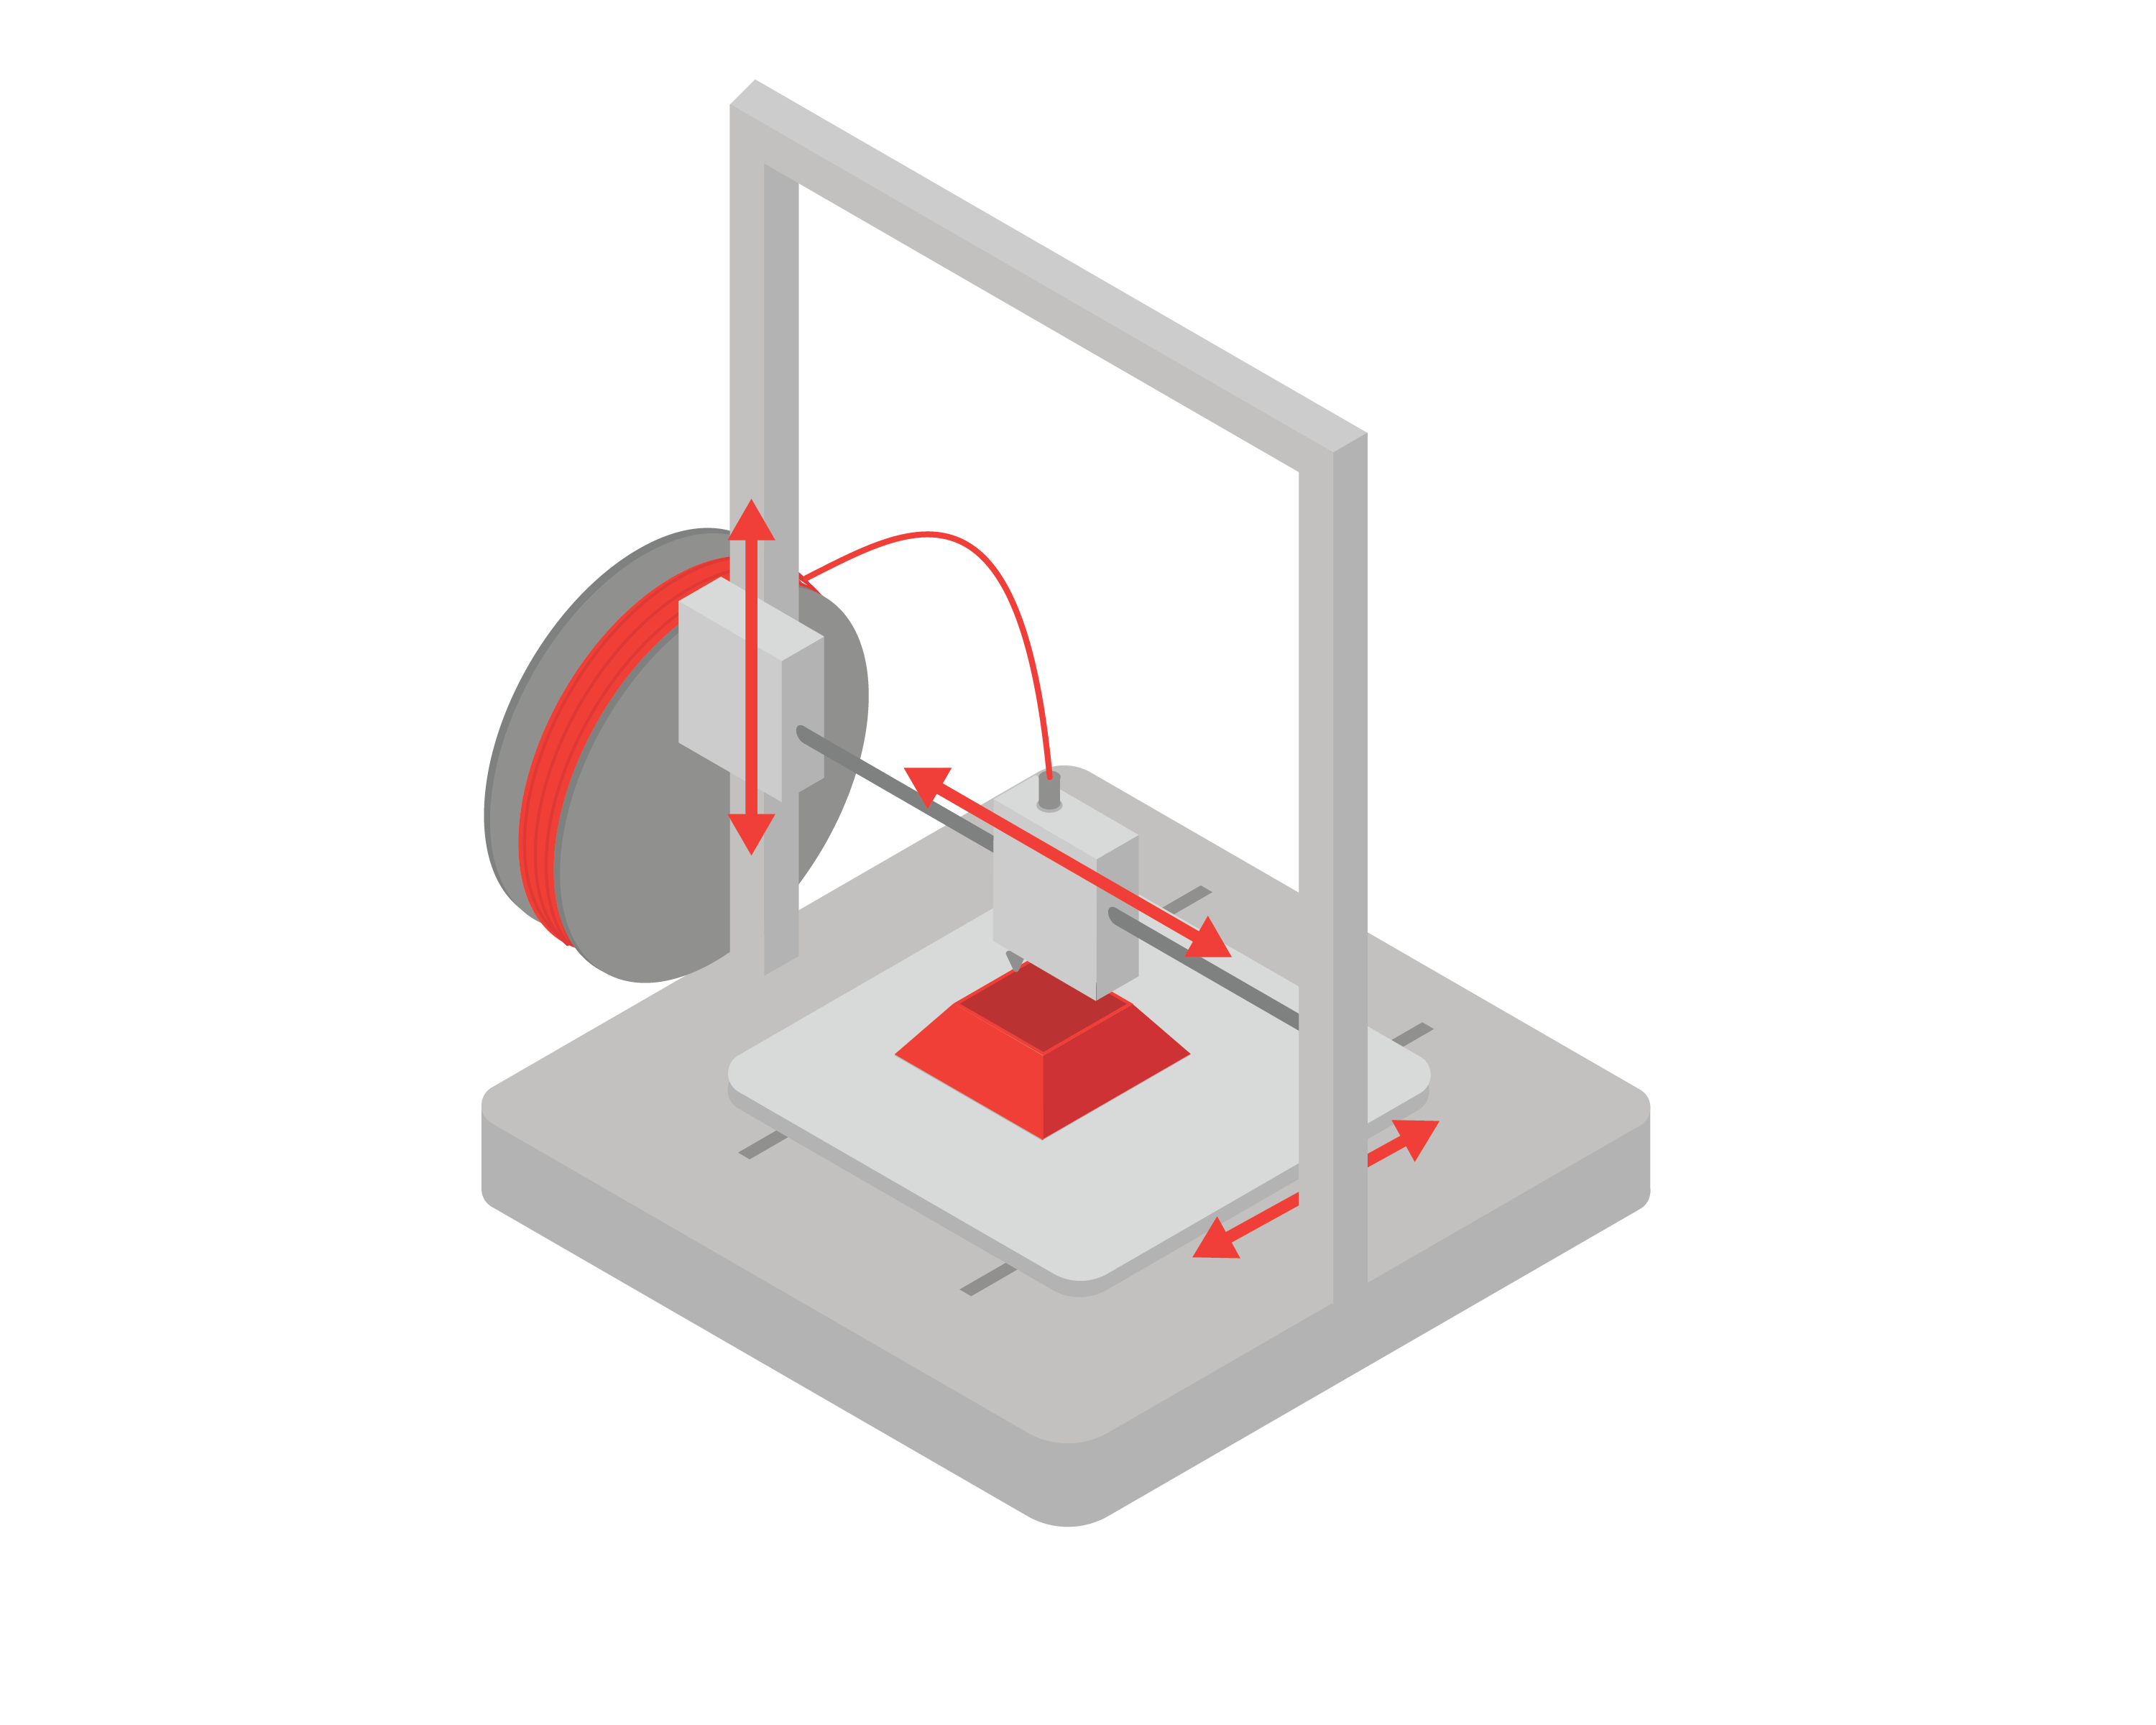
\includegraphics[width=.75\textwidth]{3dprinter.png}


\section{Laser Cutting}

Similarly, another manufacturing method enabled by new technologies is laser cutting. Like 3D printing it has come into prominence as a method to quickly prototype parts, however it is not an additive manufacturing process.

Instead laser cutting uses a laser beam to cut and etch through sheets of plastic, however it can also be used for other materials such as fabrics and card stocks. Laser cutting is mostly limited by material thickness, and as such can only cut through thinner sheets of material.

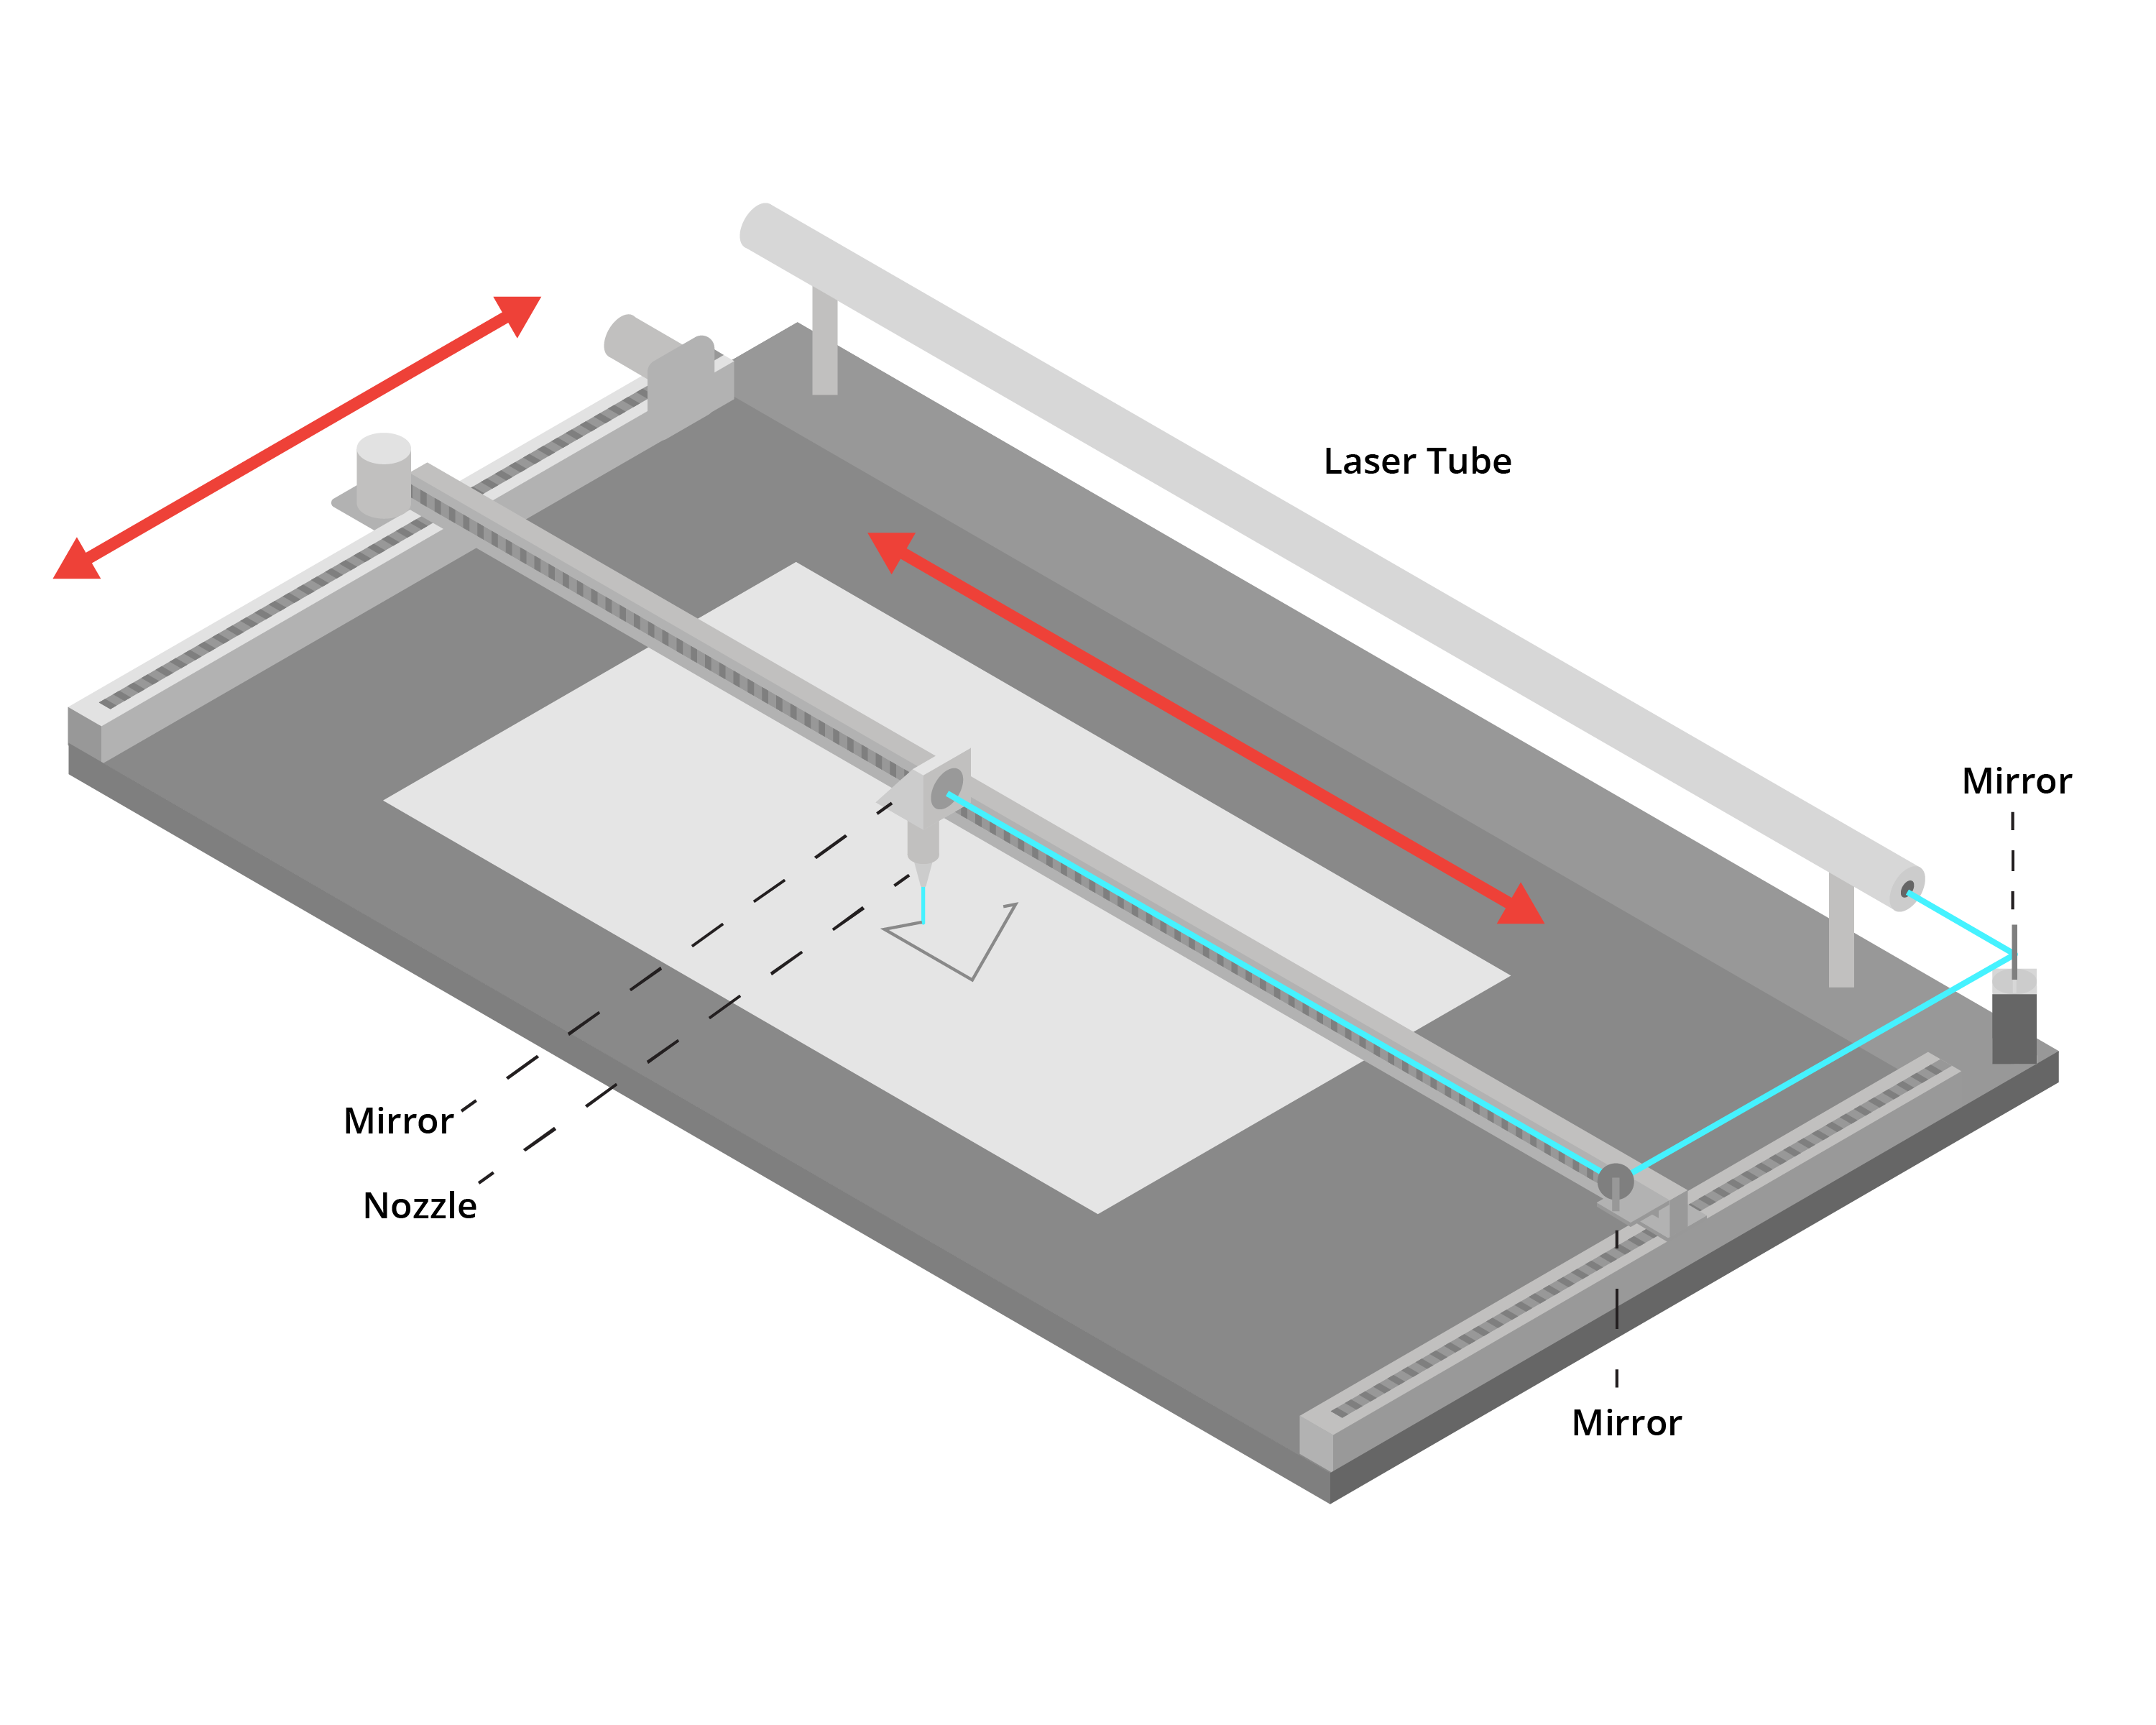
\includegraphics[width=.75\textwidth]{laserCutter.png}

%laser cutting graphic